\documentclass[12pt]{article}
\usepackage{graphicx}
\usepackage{caption}
\usepackage[semicolon]{natbib}
\usepackage{authblk}
\usepackage[utf8]{inputenc}
\usepackage[margin=2.5cm]{geometry}
\usepackage{setspace}
\usepackage{tabularx}
\usepackage{xltabular}
\usepackage{booktabs}
\usepackage{longtable}
\usepackage{rotating}
% \usepackage{float}
\usepackage[british]{datetime2}
%\usepackage{float}
\usepackage[labelsep=period]{caption}
\captionsetup[table]{name=Table}
\renewcommand{\thetable}{\Roman{table}}
\renewcommand\Affilfont{\itshape\small}

\title{Artificial States and Civil Conflict Revisited}
\author[1]{Marius Swane Wishman}
\author[1]{Charles Butcher}
\affil[1]{Department of Sociology and Political Science, NTNU}
\date{}

\providecommand{\keywords}[1]
{
  \small	
  \textbf{\textit{Keywords---}} #1
}

%\linespread{1.5}

\begin{document}


\tableofcontents

\pagebreak

\singlespacing


\section{Appendix}

\subsection{Main Results: Armed conflict onset rate}

    
\begin{table}[H]
\begin{center}
\scalebox{0.7}{
\begin{tabular}{l c c}
\hline
 & Baseline & Geography and climate \\
\hline
Log ISD states                    & $0.03^{**}$ & $0.03^{*}$     \\
                                  & $(0.01)$    & $(0.01)$       \\
Log mean EPR groups               & $0.04^{**}$ & $0.04^{**}$    \\
                                  & $(0.01)$    & $(0.01)$       \\
Log population density in 1500    & $0.00$      & $-0.00$        \\
                                  & $(0.01)$    & $(0.01)$       \\
Former colony                     & $-0.00$     & $-0.00$        \\
                                  & $(0.02)$    & $(0.03)$       \\
Historical conflict               & $-0.03$     & $-0.03$        \\
                                  & $(0.07)$    & $(0.08)$       \\
Neolithic revolution              & $0.00$      & $0.00$         \\
                                  & $(0.00)$    & $(0.00)$       \\
Area                              & $0.00$      & $0.00$         \\
                                  & $(0.00)$    & $(0.00)$       \\
Ethnic fractionalization          & $0.00$      & $-0.02$        \\
                                  & $(0.03)$    & $(0.04)$       \\
Perc. Rugged                      &             & $0.01$         \\
                                  &             & $(0.01)$       \\
Log agricultural suitability      &             & $0.00$         \\
                                  &             & $(0.01)$       \\
Log exported slaves by land area  & $0.00$      & $0.00$         \\
                                  & $(0.00)$    & $(0.00)$       \\
Latin America and the Caribbean   & $0.02$      & $-0.00$        \\
                                  & $(0.03)$    & $(0.03)$       \\
The Middle East and Nother Africa & $0.03$      & $0.04$         \\
                                  & $(0.02)$    & $(0.03)$       \\
Sub-Saharan Africa                & $0.02$      & $0.01$         \\
                                  & $(0.03)$    & $(0.04)$       \\
Western Europe and North America  & $-0.01$     & $-0.02$        \\
                                  & $(0.02)$    & $(0.03)$       \\
Asia and Pacific                  & $0.05^{*}$  & $0.05^{\cdot}$ \\
                                  & $(0.02)$    & $(0.03)$       \\
Log absolute latitude             & $0.00$      & $-0.00$        \\
                                  & $(0.01)$    & $(0.01)$       \\
Desert (middle latitude)          &             & $-0.05$        \\
                                  &             & $(0.05)$       \\
Landlocked                        &             & $-0.00$        \\
                                  &             & $(0.02)$       \\
Island                            &             & $-0.00$        \\
                                  &             & $(0.03)$       \\
\hline
R$^2$                             & $0.32$      & $0.33$         \\
Adj. R$^2$                        & $0.24$      & $0.22$         \\
Num. obs.                         & $151$       & $134$          \\
\hline
\multicolumn{3}{l}{\scriptsize{Reference region is Eastern Europe and Central Asia.}}
\end{tabular}
}
\caption{Armed conflict onset rate}
\label{onsets}
\end{center}
\end{table}

    
\clearpage    

\subsection{Main Results: Armed conflict onset rate, Government}

    
\begin{table}[H]
\begin{center}
\scalebox{0.7}{
\begin{tabular}{l c c}
\hline
 & Baseline & Geography and climate \\
\hline
Log ISD states                    & $0.01^{**}$     & $0.01^{*}$     \\
                                  & $(0.00)$        & $(0.00)$       \\
Log mean EPR groups               & $0.01^{\cdot}$  & $0.01$         \\
                                  & $(0.00)$        & $(0.00)$       \\
Log population density in 1500    & $0.00$          & $-0.00$        \\
                                  & $(0.00)$        & $(0.00)$       \\
Former colony                     & $-0.01$         & $-0.00$        \\
                                  & $(0.01)$        & $(0.01)$       \\
Historical conflict               & $-0.04$         & $-0.02$        \\
                                  & $(0.03)$        & $(0.03)$       \\
Neolithic revolution              & $0.00$          & $0.00$         \\
                                  & $(0.00)$        & $(0.00)$       \\
Area                              & $0.00$          & $0.00$         \\
                                  & $(0.00)$        & $(0.00)$       \\
Ethnic fractionalization          & $0.00$          & $-0.01$        \\
                                  & $(0.01)$        & $(0.02)$       \\
Perc. Rugged                      &                 & $0.00$         \\
                                  &                 & $(0.00)$       \\
Log agricultural suitability      &                 & $0.00$         \\
                                  &                 & $(0.00)$       \\
Log exported slaves by land area  & $-0.00$         & $-0.00$        \\
                                  & $(0.00)$        & $(0.00)$       \\
Latin America and the Caribbean   & $0.01$          & $0.00$         \\
                                  & $(0.01)$        & $(0.01)$       \\
The Middle East and Nother Africa & $0.02^{\cdot}$  & $0.02^{\cdot}$ \\
                                  & $(0.01)$        & $(0.01)$       \\
Sub-Saharan Africa                & $0.01$          & $0.01$         \\
                                  & $(0.01)$        & $(0.01)$       \\
Western Europe and North America  & $-0.01$         & $-0.00$        \\
                                  & $(0.01)$        & $(0.01)$       \\
Asia and Pacific                  & $0.00$          & $0.00$         \\
                                  & $(0.01)$        & $(0.01)$       \\
Log absolute latitude             & $-0.01^{\cdot}$ & $-0.01^{**}$   \\
                                  & $(0.00)$        & $(0.00)$       \\
Desert (middle latitude)          &                 & $-0.01$        \\
                                  &                 & $(0.02)$       \\
Landlocked                        &                 & $0.01$         \\
                                  &                 & $(0.01)$       \\
Island                            &                 & $-0.00$        \\
                                  &                 & $(0.01)$       \\
\hline
R$^2$                             & $0.29$          & $0.34$         \\
Adj. R$^2$                        & $0.22$          & $0.22$         \\
Num. obs.                         & $151$           & $134$          \\
\hline
\multicolumn{3}{l}{\scriptsize{Reference region is Eastern Europe and Central Asia.}}
\end{tabular}
}
\caption{Onset of conflicts over government}
\label{onsetgov}
\end{center}
\end{table}

    
        
\clearpage    
  
\subsection{Main Results: Armed conflict onset rate, Territory}

    
\begin{table}[H]
\begin{center}
\scalebox{0.7}{
\begin{tabular}{l c c}
\hline
 & Baseline & Geography and climate \\
\hline
Log ISD states                    & $0.02^{*}$  & $0.02^{*}$     \\
                                  & $(0.01)$    & $(0.01)$       \\
Log mean EPR groups               & $0.03^{**}$ & $0.04^{**}$    \\
                                  & $(0.01)$    & $(0.01)$       \\
Log population density in 1500    & $0.00$      & $0.00$         \\
                                  & $(0.01)$    & $(0.01)$       \\
Former colony                     & $0.00$      & $-0.00$        \\
                                  & $(0.02)$    & $(0.02)$       \\
Historical conflict               & $0.01$      & $-0.01$        \\
                                  & $(0.06)$    & $(0.07)$       \\
Neolithic revolution              & $0.00$      & $0.00$         \\
                                  & $(0.00)$    & $(0.00)$       \\
Area                              & $0.00$      & $0.00$         \\
                                  & $(0.00)$    & $(0.00)$       \\
Ethnic fractionalization          & $-0.00$     & $-0.02$        \\
                                  & $(0.03)$    & $(0.04)$       \\
Perc. Rugged                      &             & $0.00$         \\
                                  &             & $(0.01)$       \\
Log agricultural suitability      &             & $0.00$         \\
                                  &             & $(0.01)$       \\
Log exported slaves by land area  & $0.00$      & $0.00$         \\
                                  & $(0.00)$    & $(0.00)$       \\
Latin America and the Caribbean   & $0.01$      & $-0.01$        \\
                                  & $(0.02)$    & $(0.03)$       \\
The Middle East and Nother Africa & $0.02$      & $0.02$         \\
                                  & $(0.02)$    & $(0.03)$       \\
Sub-Saharan Africa                & $0.01$      & $-0.00$        \\
                                  & $(0.03)$    & $(0.03)$       \\
Western Europe and North America  & $-0.01$     & $-0.01$        \\
                                  & $(0.02)$    & $(0.02)$       \\
Asia and Pacific                  & $0.05^{*}$  & $0.05^{\cdot}$ \\
                                  & $(0.02)$    & $(0.02)$       \\
Log absolute latitude             & $0.01$      & $0.01$         \\
                                  & $(0.01)$    & $(0.01)$       \\
Desert (middle latitude)          &             & $-0.05$        \\
                                  &             & $(0.04)$       \\
Landlocked                        &             & $-0.01$        \\
                                  &             & $(0.02)$       \\
Island                            &             & $-0.00$        \\
                                  &             & $(0.03)$       \\
\hline
R$^2$                             & $0.27$      & $0.31$         \\
Adj. R$^2$                        & $0.19$      & $0.18$         \\
Num. obs.                         & $151$       & $134$          \\
\hline
\multicolumn{3}{l}{\scriptsize{Reference region is Eastern Europe and Central Asia.}}
\end{tabular}
}
\caption{Onset of conflicts over territory}
\label{onsetterr}
\end{center}
\end{table}

    
    
\clearpage        

\subsection{Main Results: Armed conflict onset rate, 1946-1988}

    
\begin{table}[H]
\begin{center}
\scalebox{0.8}{
\begin{tabular}{l c c}
\hline
 & Baseline & Geography and climate \\
\hline
Log ISD states                    & $0.03^{***}$   & $0.03^{***}$   \\
                                  & $(0.01)$       & $(0.01)$       \\
Log mean EPR groups               & $0.02^{*}$     & $0.02^{\cdot}$ \\
                                  & $(0.01)$       & $(0.01)$       \\
Log population density in 1500    & $-0.00$        & $-0.01$        \\
                                  & $(0.00)$       & $(0.01)$       \\
Former colony                     & $-0.01$        & $-0.02$        \\
                                  & $(0.01)$       & $(0.02)$       \\
Historical conflict               & $0.04$         & $0.03$         \\
                                  & $(0.05)$       & $(0.05)$       \\
Neolithic revolution              & $-0.00$        & $-0.00$        \\
                                  & $(0.00)$       & $(0.00)$       \\
Area                              & $-0.00$        & $-0.00$        \\
                                  & $(0.00)$       & $(0.00)$       \\
Ethnic fractionalization          & $0.00$         & $0.01$         \\
                                  & $(0.02)$       & $(0.03)$       \\
Perc. Rugged                      &                & $-0.00$        \\
                                  &                & $(0.01)$       \\
Log agricultural suitability      &                & $0.01$         \\
                                  &                & $(0.01)$       \\
Log exported slaves by land area  & $0.00$         & $-0.00$        \\
                                  & $(0.00)$       & $(0.00)$       \\
Latin America and the Caribbean   & $0.04^{\cdot}$ & $0.02$         \\
                                  & $(0.02)$       & $(0.03)$       \\
The Middle East and Nother Africa & $0.05^{*}$     & $0.06^{*}$     \\
                                  & $(0.02)$       & $(0.03)$       \\
Sub-Saharan Africa                & $0.03$         & $0.03$         \\
                                  & $(0.03)$       & $(0.03)$       \\
Western Europe and North America  & $0.02$         & $0.01$         \\
                                  & $(0.02)$       & $(0.02)$       \\
Asia and Pacific                  & $0.07^{**}$    & $0.07^{**}$    \\
                                  & $(0.02)$       & $(0.02)$       \\
Log absolute latitude             & $-0.00$        & $-0.01$        \\
                                  & $(0.01)$       & $(0.01)$       \\
Desert (middle latitude)          &                & $0.03$         \\
                                  &                & $(0.04)$       \\
Landlocked                        &                & $-0.02$        \\
                                  &                & $(0.01)$       \\
Island                            &                & $-0.01$        \\
                                  &                & $(0.02)$       \\
\hline
R$^2$                             & $0.40$         & $0.44$         \\
Adj. R$^2$                        & $0.32$         & $0.32$         \\
Num. obs.                         & $129$          & $114$          \\
\hline
\multicolumn{3}{l}{\scriptsize{Reference region is Eastern Europe and Central Asia.}}
\end{tabular}
}
\caption{Armed conflict onset rate, 1946-1988}
\label{onset46-88}
\end{center}
\end{table}

 
    
\clearpage     
  
\subsection{Main Results: Armed conflict onset rate, 1989-2000}

    
\begin{table}[H]
\begin{center}
\scalebox{0.8}{
\begin{tabular}{l c c}
\hline
 & Baseline & Geography and climate \\
\hline
Log ISD states                    & $0.05^{*}$  & $0.05^{\cdot}$ \\
                                  & $(0.02)$    & $(0.03)$       \\
Log mean EPR groups               & $0.07^{**}$ & $0.09^{**}$    \\
                                  & $(0.03)$    & $(0.03)$       \\
Log population density in 1500    & $0.02$      & $0.02$         \\
                                  & $(0.01)$    & $(0.02)$       \\
Former colony                     & $-0.04$     & $-0.05$        \\
                                  & $(0.05)$    & $(0.06)$       \\
Historical conflict               & $-0.16$     & $-0.18$        \\
                                  & $(0.16)$    & $(0.18)$       \\
Neolithic revolution              & $-0.00$     & $0.00$         \\
                                  & $(0.00)$    & $(0.00)$       \\
Area                              & $0.01$      & $0.02$         \\
                                  & $(0.01)$    & $(0.01)$       \\
Ethnic fractionalization          & $-0.02$     & $-0.07$        \\
                                  & $(0.08)$    & $(0.10)$       \\
Perc. Rugged                      &             & $0.02$         \\
                                  &             & $(0.02)$       \\
Log agricultural suitability      &             & $0.00$         \\
                                  &             & $(0.02)$       \\
Log exported slaves by land area  & $-0.00$     & $0.00$         \\
                                  & $(0.01)$    & $(0.01)$       \\
Latin America and the Caribbean   & $0.04$      & $0.02$         \\
                                  & $(0.06)$    & $(0.07)$       \\
The Middle East and Nother Africa & $0.05$      & $0.04$         \\
                                  & $(0.06)$    & $(0.08)$       \\
Sub-Saharan Africa                & $0.04$      & $0.02$         \\
                                  & $(0.07)$    & $(0.09)$       \\
Western Europe and North America  & $-0.05$     & $-0.07$        \\
                                  & $(0.06)$    & $(0.07)$       \\
Asia and Pacific                  & $0.09$      & $0.07$         \\
                                  & $(0.06)$    & $(0.06)$       \\
Log absolute latitude             & $0.02$      & $0.02$         \\
                                  & $(0.02)$    & $(0.02)$       \\
Desert (middle latitude)          &             & $-0.16$        \\
                                  &             & $(0.12)$       \\
Landlocked                        &             & $-0.01$        \\
                                  &             & $(0.04)$       \\
Island                            &             & $0.01$         \\
                                  &             & $(0.07)$       \\
\hline
R$^2$                             & $0.24$      & $0.27$         \\
Adj. R$^2$                        & $0.15$      & $0.14$         \\
Num. obs.                         & $151$       & $134$          \\
\hline
\multicolumn{3}{l}{\scriptsize{Reference region is Eastern Europe and Central Asia.}}
\end{tabular}
}
\caption{Armed conflict onset: 1989-2000}
\label{onset89-20}
\end{center}
\end{table}

    
    
\clearpage    


\subsection{Main Results: Armed conflict onset rate, 2001-2019}

    
\begin{table}[H]
\begin{center}
\scalebox{0.7}{
\begin{tabular}{l c c}
\hline
 & Baseline & Geography and climate \\
\hline
Log ISD states                    & $0.03^{*}$  & $0.03^{\cdot}$ \\
                                  & $(0.01)$    & $(0.01)$       \\
Log mean EPR groups               & $0.03^{*}$  & $0.04^{*}$     \\
                                  & $(0.01)$    & $(0.02)$       \\
Log population density in 1500    & $0.01$      & $0.01$         \\
                                  & $(0.01)$    & $(0.01)$       \\
Former colony                     & $0.02$      & $0.02$         \\
                                  & $(0.03)$    & $(0.03)$       \\
Historical conflict               & $-0.05$     & $-0.04$        \\
                                  & $(0.09)$    & $(0.10)$       \\
Neolithic revolution              & $0.00$      & $0.00$         \\
                                  & $(0.00)$    & $(0.00)$       \\
Area                              & $0.00$      & $0.01$         \\
                                  & $(0.01)$    & $(0.01)$       \\
Ethnic fractionalization          & $0.03$      & $-0.01$        \\
                                  & $(0.04)$    & $(0.05)$       \\
Perc. Rugged                      &             & $-0.00$        \\
                                  &             & $(0.01)$       \\
Log agricultural suitability      &             & $-0.00$        \\
                                  &             & $(0.01)$       \\
Log exported slaves by land area  & $0.00$      & $0.00$         \\
                                  & $(0.00)$    & $(0.01)$       \\
Latin America and the Caribbean   & $0.02$      & $0.02$         \\
                                  & $(0.03)$    & $(0.04)$       \\
The Middle East and Nother Africa & $0.09^{**}$ & $0.10^{*}$     \\
                                  & $(0.03)$    & $(0.04)$       \\
Sub-Saharan Africa                & $0.05$      & $0.05$         \\
                                  & $(0.04)$    & $(0.05)$       \\
Western Europe and North America  & $0.01$      & $0.01$         \\
                                  & $(0.03)$    & $(0.04)$       \\
Asia and Pacific                  & $0.07^{*}$  & $0.08^{*}$     \\
                                  & $(0.03)$    & $(0.04)$       \\
Log absolute latitude             & $0.01$      & $0.00$         \\
                                  & $(0.01)$    & $(0.01)$       \\
Desert (middle latitude)          &             & $-0.08$        \\
                                  &             & $(0.06)$       \\
Landlocked                        &             & $0.01$         \\
                                  &             & $(0.02)$       \\
Island                            &             & $-0.02$        \\
                                  &             & $(0.04)$       \\
\hline
R$^2$                             & $0.29$      & $0.30$         \\
Adj. R$^2$                        & $0.21$      & $0.18$         \\
Num. obs.                         & $151$       & $134$          \\
\hline
\multicolumn{3}{l}{\scriptsize{Reference region is Eastern Europe and Central Asia.}}
\end{tabular}
}
\caption{Armed conflict onset rate, 2001-2019}
\label{onsets0119}
\end{center}
\end{table}

    
    
\clearpage    

\subsection{Alternative Measures of State History}

    
\begin{table}[H]
\begin{center}
\scalebox{0.7}{
\begin{tabular}{l c c c c}
\hline
 & Wig 2016 JH & Paine 2019 SLPCS & State antiquity AD & Fractal index \\
\hline
Log ISD states                    & $0.05^{**}$ & $0.04^{**}$     & $0.02^{*}$     & $0.03^{**}$ \\
                                  & $(0.02)$    & $(0.01)$        & $(0.01)$       & $(0.01)$    \\
Sum eth. groups with JH $>$ 2     & $-0.02$     &                 &                &             \\
                                  & $(0.01)$    &                 &                &             \\
Log sum SLPCS groups              &             & $-0.02$         &                &             \\
                                  &             & $(0.02)$        &                &             \\
Log sum PCS groups                &             & $0.01$          &                &             \\
                                  &             & $(0.03)$        &                &             \\
Mean State Antiquity, 0 AD - 1800 &             &                 & $0.00^{\cdot}$ &             \\
                                  &             &                 & $(0.00)$       &             \\
Alesina et al fractal index       &             &                 &                & $0.00$      \\
                                  &             &                 &                & $(0.03)$    \\
Log mean EPR groups               & $0.02$      & $-0.01$         & $0.04^{**}$    & $0.03^{**}$ \\
                                  & $(0.03)$    & $(0.02)$        & $(0.01)$       & $(0.01)$    \\
Log population density in 1500    & $0.01$      & $0.00$          & $-0.00$        & $0.00$      \\
                                  & $(0.01)$    & $(0.01)$        & $(0.01)$       & $(0.01)$    \\
Former colony                     &             &                 & $0.00$         & $0.00$      \\
                                  &             &                 & $(0.02)$       & $(0.02)$    \\
Historical conflict               & $0.17$      & $0.68^{**}$     & $-0.03$        & $-0.02$     \\
                                  & $(0.18)$    & $(0.22)$        & $(0.07)$       & $(0.07)$    \\
Neolithic revolution              & $-0.00$     & $-0.00$         & $-0.00$        & $0.00$      \\
                                  & $(0.00)$    & $(0.00)$        & $(0.00)$       & $(0.00)$    \\
Area                              & $0.04$      & $0.03$          & $0.00$         & $0.00$      \\
                                  & $(0.03)$    & $(0.02)$        & $(0.00)$       & $(0.00)$    \\
Ethnic fractionalization          & $-0.03$     & $-0.07$         & $-0.00$        &             \\
                                  & $(0.07)$    & $(0.06)$        & $(0.04)$       &             \\
Log exported slaves by land area  & $-0.00$     & $0.00$          & $0.00$         & $0.00$      \\
                                  & $(0.00)$    & $(0.00)$        & $(0.00)$       & $(0.00)$    \\
Latin America and the Caribbean   &             &                 & $0.01$         & $0.02$      \\
                                  &             &                 & $(0.03)$       & $(0.03)$    \\
The Middle East and Nother Africa &             &                 & $0.02$         & $0.03$      \\
                                  &             &                 & $(0.03)$       & $(0.02)$    \\
Sub-Saharan Africa                &             &                 & $0.03$         & $0.02$      \\
                                  &             &                 & $(0.03)$       & $(0.03)$    \\
Western Europe and North America  &             &                 & $-0.02$        & $-0.02$     \\
                                  &             &                 & $(0.03)$       & $(0.02)$    \\
Asia and Pacific                  &             &                 & $0.03$         & $0.05^{*}$  \\
                                  &             &                 & $(0.03)$       & $(0.02)$    \\
Log absolute latitude             & $-0.02$     & $-0.02^{\cdot}$ & $-0.00$        & $0.01$      \\
                                  & $(0.01)$    & $(0.01)$        & $(0.01)$       & $(0.01)$    \\
\hline
R$^2$                             & $0.63$      & $0.77$          & $0.34$         & $0.31$      \\
Adj. R$^2$                        & $0.48$      & $0.66$          & $0.25$         & $0.23$      \\
Num. obs.                         & $36$        & $35$            & $139$          & $149$       \\
\hline
\multicolumn{5}{l}{\scriptsize{Reference region is Eastern Europe and Central Asia.}}
\end{tabular}
}
\caption{Alternative explenations}
\label{StateHistoryTable}
\end{center}
\end{table}

    

    
\clearpage    


\subsection{Regional Subsets}

    
\begin{sidewaystable}
\begin{center}
\scalebox{0.6}{
\begin{tabular}{l c c c c c c c c c}
\hline
 & SSA & Asia & Latin America & MENA & East. Europe and Central Asia & West & Former colonies & Non-West & Early Col. Dropped \\
\hline
Log ISD states                    & $0.03^{*}$     & $0.02$         & $0.01$   & $0.02$   & $-0.08$  & $-0.00$  & $0.02^{*}$     & $0.03^{**}$    & $0.03^{**}$  \\
                                  & $(0.01)$       & $(0.04)$       & $(0.01)$ & $(0.04)$ & $(0.05)$ & $(0.00)$ & $(0.01)$       & $(0.01)$       & $(0.01)$     \\
Log mean EPR groups               & $-0.00$        & $0.22^{*}$     & $-0.01$  & $0.01$   & $0.05$   & $0.00$   & $0.04^{***}$   & $0.04^{**}$    & $0.04^{***}$ \\
                                  & $(0.01)$       & $(0.07)$       & $(0.01)$ & $(0.04)$ & $(0.04)$ & $(0.00)$ & $(0.01)$       & $(0.01)$       & $(0.01)$     \\
Log population density in 1500    & $0.01$         & $-0.00$        & $0.00$   & $0.02$   & $-0.01$  & $-0.00$  & $0.01$         & $0.00$         & $0.00$       \\
                                  & $(0.01)$       & $(0.04)$       & $(0.01)$ & $(0.03)$ & $(0.02)$ & $(0.00)$ & $(0.01)$       & $(0.01)$       & $(0.01)$     \\
Former colony                     & $-0.05$        & $0.23^{\cdot}$ &          & $-0.13$  & $0.05$   & $-0.00$  &                & $0.02$         & $0.01$       \\
                                  & $(0.03)$       & $(0.10)$       &          & $(0.10)$ & $(0.09)$ & $(0.01)$ &                & $(0.03)$       & $(0.02)$     \\
Historical conflict               & $0.54^{**}$    & $0.82$         & $-0.14$  & $-0.28$  & $0.17$   & $0.03$   & $0.20^{\cdot}$ & $0.08$         & $-0.02$      \\
                                  & $(0.18)$       & $(0.59)$       & $(0.19)$ & $(0.47)$ & $(0.22)$ & $(0.02)$ & $(0.11)$       & $(0.11)$       & $(0.07)$     \\
Neolithic revolution              & $-0.00$        & $-0.00$        & $0.00$   & $-0.00$  & $0.00$   & $0.00$   & $0.00$         & $0.00$         & $0.00$       \\
                                  & $(0.00)$       & $(0.00)$       & $(0.00)$ & $(0.00)$ & $(0.00)$ & $(0.00)$ & $(0.00)$       & $(0.00)$       & $(0.00)$     \\
Area                              & $0.04^{\cdot}$ & $-0.09$        & $-0.00$  & $0.02$   & $-0.00$  & $-0.00$  & $0.00$         & $-0.00$        & $0.00$       \\
                                  & $(0.02)$       & $(0.07)$       & $(0.00)$ & $(0.04)$ & $(0.01)$ & $(0.00)$ & $(0.01)$       & $(0.01)$       & $(0.00)$     \\
Ethnic fractionalization          & $-0.03$        & $-0.01$        & $0.04$   & $0.07$   & $-0.01$  & $0.01$   & $-0.00$        & $0.01$         & $0.01$       \\
                                  & $(0.03)$       & $(0.22)$       & $(0.02)$ & $(0.10)$ & $(0.12)$ & $(0.02)$ & $(0.03)$       & $(0.04)$       & $(0.03)$     \\
Log exported slaves by land area  &                &                &          &          &          &          &                & $-0.00$        &              \\
                                  &                &                &          &          &          &          &                & $(0.00)$       &              \\
Latin America and the Caribbean   &                &                &          &          &          &          &                & $0.03$         &              \\
                                  &                &                &          &          &          &          &                & $(0.03)$       &              \\
The Middle East and Nother Africa &                &                &          &          &          &          &                & $0.04$         &              \\
                                  &                &                &          &          &          &          &                & $(0.03)$       &              \\
Sub-Saharan Africa                &                &                &          &          &          &          &                & $0.04$         &              \\
                                  &                &                &          &          &          &          &                & $(0.04)$       &              \\
Asia and Pacific                  &                &                &          &          &          &          &                & $0.05^{\cdot}$ &              \\
                                  &                &                &          &          &          &          &                & $(0.03)$       &              \\
Log absolute latitude             & $-0.01$        & $0.07$         & $0.01$   & $0.06$   & $0.00$   & $-0.00$  & $-0.01$        & $0.00$         & $-0.01$      \\
                                  & $(0.01)$       & $(0.05)$       & $(0.01)$ & $(0.26)$ & $(0.37)$ & $(0.01)$ & $(0.01)$       & $(0.01)$       & $(0.01)$     \\
\hline
R$^2$                             & $0.71$         & $0.73$         & $0.38$   & $0.68$   & $0.38$   & $0.49$   & $0.29$         & $0.31$         & $0.28$       \\
Adj. R$^2$                        & $0.63$         & $0.42$         & $0.02$   & $0.28$   & $0.06$   & $0.17$   & $0.24$         & $0.22$         & $0.23$       \\
Num. obs.                         & $42$           & $18$           & $23$     & $17$     & $27$     & $24$     & $127$          & $127$          & $146$        \\
\hline
\multicolumn{10}{l}{\scriptsize{$^{***}p<0.001$; $^{**}p<0.01$; $^{*}p<0.05$; $^{\cdot}p<0.1$}}
\end{tabular}
}
\caption{ISD states and civil war onsets by regional subsets}
\label{table:coefficients}
\end{center}
\end{sidewaystable}



    
\clearpage    

\subsection{First Stage Mediation Equations}

    
\begin{sidewaystable}[H]
\begin{center}
\scalebox{0.7}{
\begin{tabular}{l c c c c c c}
\hline
 & DV: log mean EPR groups & Log mean EPR excl. groups & GDP per capita 2000 & Relative tax capacity (2000) & Prot. missionaries & Years of colonialism \\
\hline
Log ISD states                   & $0.09$       & $0.10$         & $-0.12$         & $-0.00$    & $-0.20^{\cdot}$ & $18.02$          \\
                                 & $(0.08)$     & $(0.07)$       & $(0.12)$        & $(0.01)$   & $(0.11)$        & $(16.93)$        \\
Log population density in 1500   & $-0.02$      & $-0.03$        & $-0.09$         & $-0.01$    & $-0.17^{*}$     & $0.61$           \\
                                 & $(0.05)$     & $(0.04)$       & $(0.07)$        & $(0.01)$   & $(0.07)$        & $(12.06)$        \\
Former colony                    & $0.26$       & $0.27^{\cdot}$ & $-0.52^{\cdot}$ & $-0.02$    & $0.11$          & $66.36$          \\
                                 & $(0.17)$     & $(0.16)$       & $(0.26)$        & $(0.02)$   & $(0.33)$        & $(47.07)$        \\
Historical conflict              & $1.39^{*}$   & $1.69^{**}$    & $0.55$          & $0.01$     & $0.91$          & $397.32^{\cdot}$ \\
                                 & $(0.55)$     & $(0.52)$       & $(0.86)$        & $(0.08)$   & $(1.12)$        & $(201.42)$       \\
Neolithic revolution             & $0.00^{***}$ & $0.00^{***}$   & $0.00$          & $0.00$     & $-0.00$         & $-0.01$          \\
                                 & $(0.00)$     & $(0.00)$       & $(0.00)$        & $(0.00)$   & $(0.00)$        & $(0.01)$         \\
Area                             & $0.10^{**}$  & $0.10^{***}$   & $-0.00$         & $-0.00$    & $-0.10$         & $-24.80$         \\
                                 & $(0.03)$     & $(0.03)$       & $(0.05)$        & $(0.01)$   & $(0.08)$        & $(18.35)$        \\
Ethnic fractionalization         & $1.02^{***}$ & $0.76^{**}$    & $-0.93^{*}$     & $0.02$     & $0.13$          & $37.72$          \\
                                 & $(0.27)$     & $(0.25)$       & $(0.42)$        & $(0.04)$   & $(0.40)$        & $(72.82)$        \\
Log exported slaves by land area & $-0.01$      & $-0.04^{*}$    & $-0.14^{***}$   & $-0.00$    & $-0.05$         & $-3.25$          \\
                                 & $(0.02)$     & $(0.02)$       & $(0.04)$        & $(0.00)$   & $(0.03)$        & $(5.21)$         \\
Log absolute latitude            & $-0.17^{**}$ & $-0.12^{*}$    & $0.22^{*}$      & $0.02^{*}$ & $-0.10$         & $-10.06$         \\
                                 & $(0.06)$     & $(0.06)$       & $(0.10)$        & $(0.01)$   & $(0.09)$        & $(14.27)$        \\
\hline
R$^2$                            & $0.43$       & $0.44$         & $0.46$          & $0.15$     & $0.19$          & $0.14$           \\
Adj. R$^2$                       & $0.39$       & $0.40$         & $0.43$          & $0.08$     & $0.12$          & $0.02$           \\
Num. obs.                        & $151$        & $151$          & $150$           & $120$      & $109$           & $74$             \\
\hline
\multicolumn{7}{l}{\scriptsize{Reference region is Eastern Europe and Central Asia.}}
\end{tabular}
}
\caption{First stage mediation equations}
\label{MediationTable}
\end{center}
\end{sidewaystable}

    
    
\clearpage
 
 
\subsection{Second Stage Mediation Equations}


\clearpage
    
\begin{sidewaystable}[H]
\begin{center}
\scalebox{0.7}{
\begin{tabular}{l c c c c c c}
\hline
 & Log mean EPR groups & Log mean EPR excl. groups & GDP per capita 2000 & Relative tax capacity (2000) & Prot. missionaries & Years of colonialism \\
\hline
Log ISD states                   & $0.03^{**}$  & $0.03^{**}$  & $0.03^{***}$    & $0.03^{**}$ & $0.04^{***}$ & $0.05^{**}$ \\
                                 & $(0.01)$     & $(0.01)$     & $(0.01)$        & $(0.01)$    & $(0.01)$     & $(0.02)$    \\
Log mean EPR groups              & $0.04^{***}$ &              &                 &             &              &             \\
                                 & $(0.01)$     &              &                 &             &              &             \\
Log Mean EPR excl. groups        &              & $0.05^{***}$ &                 &             &              &             \\
                                 &              & $(0.01)$     &                 &             &              &             \\
Relative tax capacity (2000)     &              &              &                 & $-0.05$     &              &             \\
                                 &              &              &                 & $(0.09)$    &              &             \\
Log GDP per capita (2000)        &              &              & $-0.02^{***}$   &             &              &             \\
                                 &              &              & $(0.01)$        &             &              &             \\
Years of colonialism             &              &              &                 &             &              & $0.00$      \\
                                 &              &              &                 &             &              & $(0.00)$    \\
Prot. missionaries per 10,000    &              &              &                 &             & $-0.00$      &             \\
                                 &              &              &                 &             & $(0.01)$     &             \\
Log population density in 1500   & $0.00$       & $0.00$       & $-0.00$         & $0.01$      & $0.01$       & $0.01$      \\
                                 & $(0.01)$     & $(0.01)$     & $(0.00)$        & $(0.01)$    & $(0.01)$     & $(0.01)$    \\
Former colony                    & $0.01$       & $0.00$       & $-0.01$         & $0.03$      & $0.02$       & $0.02$      \\
                                 & $(0.02)$     & $(0.02)$     & $(0.02)$        & $(0.02)$    & $(0.04)$     & $(0.04)$    \\
Historical conflict              & $-0.03$      & $-0.05$      & $0.00$          & $0.03$      & $0.19$       & $0.17$      \\
                                 & $(0.07)$     & $(0.07)$     & $(0.05)$        & $(0.08)$    & $(0.12)$     & $(0.18)$    \\
Neolithic revolution             & $0.00$       & $0.00$       & $0.00^{***}$    & $0.00$      & $0.00$       & $0.00$      \\
                                 & $(0.00)$     & $(0.00)$     & $(0.00)$        & $(0.00)$    & $(0.00)$     & $(0.00)$    \\
Area                             & $0.00$       & $-0.00$      & $0.00$          & $0.00$      & $-0.00$      & $-0.00$     \\
                                 & $(0.00)$     & $(0.00)$     & $(0.00)$        & $(0.00)$    & $(0.01)$     & $(0.02)$    \\
Ethnic fractionalization         & $0.00$       & $0.01$       & $0.01$          & $0.05$      & $0.04$       & $0.06$      \\
                                 & $(0.03)$     & $(0.03)$     & $(0.03)$        & $(0.04)$    & $(0.04)$     & $(0.06)$    \\
Log exported slaves by land area & $0.00$       & $0.00$       & $-0.00$         & $-0.00$     & $-0.00$      & $-0.00$     \\
                                 & $(0.00)$     & $(0.00)$     & $(0.00)$        & $(0.00)$    & $(0.00)$     & $(0.00)$    \\
Log absolute latitude            & $-0.01$      & $-0.01$      & $-0.01^{\cdot}$ & $-0.01$     & $-0.00$      & $-0.00$     \\
                                 & $(0.01)$     & $(0.01)$     & $(0.01)$        & $(0.01)$    & $(0.01)$     & $(0.01)$    \\
\hline
R$^2$                            & $0.27$       & $0.30$       & $0.37$          & $0.24$      & $0.27$       & $0.31$      \\
Adj. R$^2$                       & $0.22$       & $0.25$       & $0.32$          & $0.17$      & $0.20$       & $0.20$      \\
Num. obs.                        & $151$        & $151$        & $150$           & $120$       & $109$        & $74$        \\
\hline
\multicolumn{7}{l}{\scriptsize{Reference region is Eastern Europe and Central Asia.}}
\end{tabular}
}
\caption{Second stage mediation equations}
\label{MediationTable2}
\end{center}
\end{sidewaystable}

\clearpage  
 

\subsection{Models with alternative dependent variables}



    
\begin{sidewaystable}[H]
\begin{center}
\scalebox{0.7}{
\begin{tabular}{l c c c c c c}
\hline
 & Ln onsets & Ln onset rate & Negbin onsets & Raw onsets & Incidence rate & War incidence rate \\
\hline
Log ISD states                    & $0.36^{***}$ & $0.00^{*}$      & $0.35^{**}$     & $2.03^{***}$   & $0.13^{*}$   & $0.03^{\cdot}$ \\
                                  & $(0.09)$     & $(0.00)$        & $(0.13)$        & $(0.57)$       & $(0.06)$     & $(0.01)$       \\
Log mean EPR groups               & $0.37^{***}$ & $0.01^{**}$     & $0.83^{***}$    & $2.27^{**}$    & $0.19^{**}$  & $0.04^{*}$     \\
                                  & $(0.10)$     & $(0.00)$        & $(0.19)$        & $(0.68)$       & $(0.07)$     & $(0.02)$       \\
Log population density in 1500    & $0.07$       & $0.00$          & $0.05$          & $0.44$         & $0.03$       & $-0.00$        \\
                                  & $(0.06)$     & $(0.00)$        & $(0.10)$        & $(0.38)$       & $(0.04)$     & $(0.01)$       \\
Former colony                     & $-0.12$      & $0.00$          & $0.08$          & $-0.74$        & $0.03$       & $0.03$         \\
                                  & $(0.21)$     & $(0.00)$        & $(0.37)$        & $(1.39)$       & $(0.13)$     & $(0.03)$       \\
Historical conflict               & $-0.23$      & $-0.00$         & $1.07$          & $-2.38$        & $-0.21$      & $0.02$         \\
                                  & $(0.64)$     & $(0.01)$        & $(1.13)$        & $(4.21)$       & $(0.41)$     & $(0.11)$       \\
Neolithic revolution              & $0.00$       & $0.00$          & $0.00$          & $0.00$         & $-0.00$      & $0.00$         \\
                                  & $(0.00)$     & $(0.00)$        & $(0.00)$        & $(0.00)$       & $(0.00)$     & $(0.00)$       \\
Area                              & $0.04$       & $0.00$          & $-0.04$         & $0.17$         & $0.00$       & $-0.00$        \\
                                  & $(0.04)$     & $(0.00)$        & $(0.07)$        & $(0.25)$       & $(0.02)$     & $(0.01)$       \\
Ethnic fractionalization          & $0.11$       & $0.00$          & $0.13$          & $0.29$         & $-0.01$      & $0.04$         \\
                                  & $(0.32)$     & $(0.01)$        & $(0.53)$        & $(2.09)$       & $(0.20)$     & $(0.05)$       \\
Log exported slaves by land area  & $0.01$       & $0.00$          & $0.02$          & $0.01$         & $0.01$       & $0.00$         \\
                                  & $(0.03)$     & $(0.00)$        & $(0.05)$        & $(0.20)$       & $(0.02)$     & $(0.01)$       \\
Latin America and the Caribbean   & $0.83^{***}$ & $0.00$          & $1.22^{**}$     & $2.90^{\cdot}$ & $0.20$       & $0.06$         \\
                                  & $(0.24)$     & $(0.01)$        & $(0.40)$        & $(1.60)$       & $(0.16)$     & $(0.04)$       \\
The Middle East and Nother Africa & $0.96^{***}$ & $0.00$          & $1.32^{***}$    & $4.30^{**}$    & $0.32^{*}$   & $0.05$         \\
                                  & $(0.23)$     & $(0.01)$        & $(0.36)$        & $(1.49)$       & $(0.14)$     & $(0.04)$       \\
Sub-Saharan Africa                & $0.73^{*}$   & $0.00$          & $1.09^{*}$      & $2.61$         & $0.17$       & $0.07$         \\
                                  & $(0.28)$     & $(0.01)$        & $(0.47)$        & $(1.86)$       & $(0.18)$     & $(0.05)$       \\
Western Europe and North America  & $-0.09$      & $-0.01^{\cdot}$ & $-0.88^{\cdot}$ & $0.24$         & $0.08$       & $0.03$         \\
                                  & $(0.22)$     & $(0.01)$        & $(0.50)$        & $(1.46)$       & $(0.14)$     & $(0.04)$       \\
Asia and Pacific                  & $0.81^{***}$ & $0.00$          & $1.22^{***}$    & $5.12^{***}$   & $0.56^{***}$ & $0.15^{***}$   \\
                                  & $(0.23)$     & $(0.01)$        & $(0.35)$        & $(1.49)$       & $(0.14)$     & $(0.04)$       \\
Log absolute latitude             & $-0.00$      & $-0.00$         & $0.01$          & $0.28$         & $0.04$       & $0.02$         \\
                                  & $(0.08)$     & $(0.00)$        & $(0.12)$        & $(0.55)$       & $(0.05)$     & $(0.01)$       \\
\hline
R$^2$                             & $0.51$       & $0.31$          & $$              & $0.38$         & $0.30$       & $0.28$         \\
Adj. R$^2$                        & $0.45$       & $0.23$          & $$              & $0.31$         & $0.22$       & $0.20$         \\
Num. obs.                         & $151$        & $151$           & $151$           & $151$          & $151$        & $151$          \\
AIC                               & $$           & $$              & $586.88$        & $$             & $$           & $$             \\
BIC                               & $$           & $$              & $638.18$        & $$             & $$           & $$             \\
Log Likelihood                    & $$           & $$              & $-276.44$       & $$             & $$           & $$             \\
Deviance                          & $$           & $$              & $158.58$        & $$             & $$           & $$             \\
\hline
\multicolumn{7}{l}{\scriptsize{Reference region is Eastern Europe and Central Asia.}}
\end{tabular}
}
\caption{Alternative dependent variables}
\label{AltDvs}
\end{center}
\end{sidewaystable}

\clearpage  


\subsection{Sensitivity test}

Figure \ref{Fig: Sens} shows how much of the variance in the conflict onset rate and the number of HSEs a potential omitted variable would have to explain in order to render the results insignificant at the $p<0.05$ level. While similar to an Imbens test, \citet{Cinelli2020} point to several important differences. This test was run on the model using the main control variables, including region fixed effects. Not even a confounder with three times the strength of the mean number of EPR ethnic groups would render the HSE results insignificant. Any omitted confounder would have to be several times stronger than the best predictors of conflict and HSEs in our models.

% This is cool, but a lot of text gets bundled on top of each other and sometimes falls outside the graph for the ln_total_epr_groups_mean. Any way you can fix that?

    \begin{figure}[!htb] \hspace{-0,5cm} 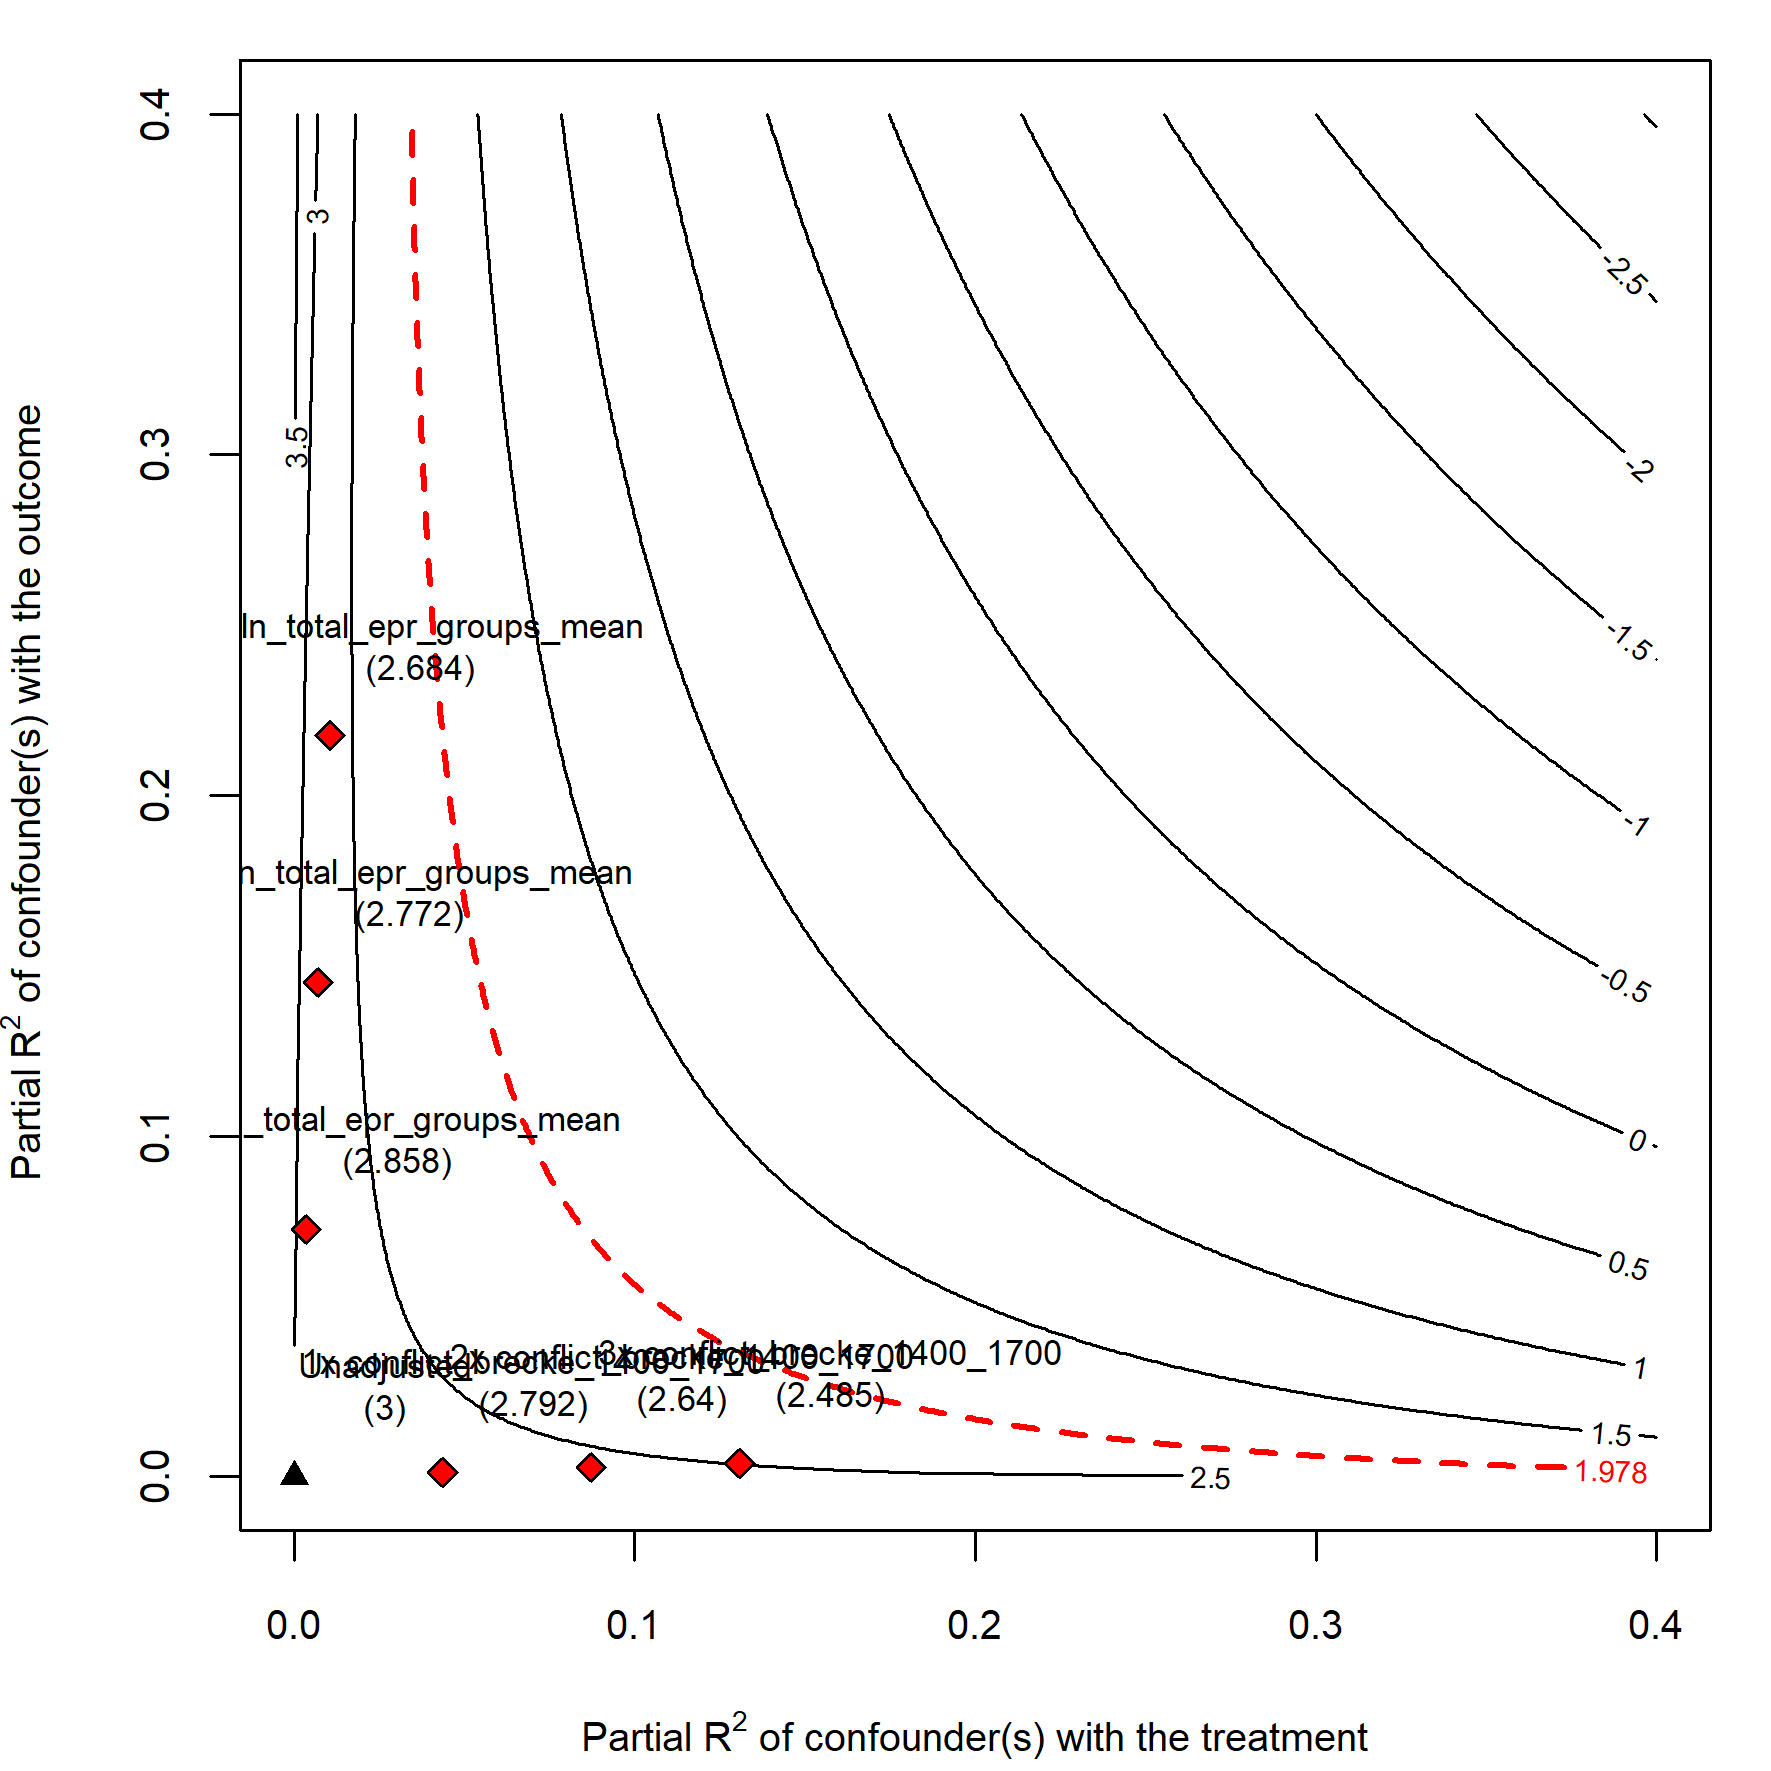
\includegraphics[width=\textwidth,
    height=\textheight, keepaspectratio]{img/hse_sens_main.png} \caption{Sensitivity test} \label{Fig: Sens} \end{figure}

\subsection{Additional tests of the state weakness mechanism}

% The reference below is not working, and I can't figure out why!
Table \ref{MediationRob} shows associations between the number of ISD states and alternative measures of state weakness to further explore these mechanisms. We use the ``State authority over territory" (Territorial capacity), ``State fiscal source of revenue" (Fiscal capacity) and ``Criteria for appointment decisions in the state administration" (Administrative capacity) variables from the VDEM dataset \citep{Coppedge2021} as indicators of various dimensions of state capacity. The territorial capacity variable captures the extent to which states control their territories. Higher scores on the fiscal capacity variable indicate movements towards direct taxation of property or income. Lower scores indicate the inability to generate taxation revenue or dependence on natural resource extraction or international aid. Higher scores on the administrative capacity variable indicate movements towards an increasingly impartial recruitment to the bureaucracy based on merit rather than personal ties or patronage. We also test the average GDP level over the 1946-2018 period and the average Polyarchy score over the same period.   

Although each of these variables represents a potential alternative mediator, we only show the first-stage equations here. None of these measures of state weakness are highly correlated with the number of ISD states between 1816-1920 and thus do not represent strong contenders for mediators. Overall, we see this as an indication that the links between ISD states and modern internal conflict rates are not well explained by the state weakness mechanism, at least on the country level. 

 \clearpage     


\begin{sidewaystable}[H]
\begin{center}
\scalebox{0.7}{
\begin{tabular}{l c c c c c}
\hline
 & DV: Mean Territorial Capacity & Mean Fiscal Cap.  & Mean Admin. Cap. & Mean GDP per capita & Mean polyarchy score \\
\hline
Log ISD states                   & $-1.26$         & $0.22^{\cdot}$ & $0.11$       & $-0.12$         & $0.03$          \\
                                 & $(1.02)$        & $(0.12)$       & $(0.12)$     & $(0.11)$        & $(0.03)$        \\
Log population density in 1500   & $0.42$          & $0.17^{*}$     & $0.15^{*}$   & $-0.11^{\cdot}$ & $0.05^{**}$     \\
                                 & $(0.64)$        & $(0.08)$       & $(0.07)$     & $(0.07)$        & $(0.02)$        \\
Former colony                    & $-2.51$         & $-0.81^{**}$   & $-0.70^{**}$ & $-0.54^{*}$     & $-0.16^{**}$    \\
                                 & $(2.30)$        & $(0.28)$       & $(0.26)$     & $(0.24)$        & $(0.06)$        \\
Historical conflict              & $-0.29$         & $-1.20$        & $-0.73$      & $0.29$          & $-0.34^{\cdot}$ \\
                                 & $(7.44)$        & $(0.89)$       & $(0.85)$     & $(0.78)$        & $(0.19)$        \\
Neolithic revolution             & $-0.00$         & $-0.00^{*}$    & $-0.00^{**}$ & $0.00^{*}$      & $-0.00^{***}$   \\
                                 & $(0.00)$        & $(0.00)$       & $(0.00)$     & $(0.00)$        & $(0.00)$        \\
Area                             & $0.23$          & $0.09^{\cdot}$ & $0.05$       & $0.00$          & $0.01$          \\
                                 & $(0.43)$        & $(0.05)$       & $(0.05)$     & $(0.05)$        & $(0.01)$        \\
Ethnic fractionalization         & $-2.57$         & $-1.08^{*}$    & $-0.26$      & $-0.46$         & $-0.15$         \\
                                 & $(3.63)$        & $(0.44)$       & $(0.42)$     & $(0.38)$        & $(0.09)$        \\
Log exported slaves by land area & $-0.63^{\cdot}$ & $-0.04$        & $-0.06$      & $-0.12^{***}$   & $-0.01$         \\
                                 & $(0.32)$        & $(0.04)$       & $(0.04)$     & $(0.03)$        & $(0.01)$        \\
Log absolute latitude            & $1.72^{*}$      & $0.28^{**}$    & $0.20^{*}$   & $0.23^{*}$      & $0.10^{***}$    \\
                                 & $(0.85)$        & $(0.10)$       & $(0.10)$     & $(0.09)$        & $(0.02)$        \\
\hline
R$^2$                            & $0.19$          & $0.34$         & $0.21$       & $0.45$          & $0.37$          \\
Adj. R$^2$                       & $0.13$          & $0.29$         & $0.16$       & $0.41$          & $0.33$          \\
Num. obs.                        & $151$           & $151$          & $151$        & $151$           & $151$           \\
\hline
\multicolumn{6}{l}{\scriptsize{Averages are measured over the 1946-2020 period (1946-2018 for GDP per capita)}}
\end{tabular}
}
\caption{First stage equations}
\label{MediationTableRob}
\end{center}
\end{sidewaystable}

    
 \clearpage     

\subsection{Secessionism}

Here we explore the extent to which the main results reflect an increase in the risk of secessionist movements. The UCDP data differentiates between conflicts with ``governmental'' and ``territorial'' incompatibilities, but does not specifically identify secessionist movements (although these are a subset of territorial conflicts). We use data from Griffiths (2016) on secessionist movements active in independent states after 1946 to unpack the relationship between HSEs and secessionism further.  


    
% Table created by stargazer v.5.2.2 by Marek Hlavac, Harvard University. E-mail: hlavac at fas.harvard.edu
% Date and time: ons., feb 09, 2022 - 08:41:36
\begin{table}[!htbp] \centering 
  \caption{Descriptive Statistics: HSEs and secessionist movements} 
  \label{Tab: Sec_Desc} 
\begin{tabular}{@{\extracolsep{5pt}} ccccc} 
\\[-1.8ex]\hline 
\hline \\[-1.8ex] 
HSEs & Onset rate & Incidence rate & Ratio V/NV years & N \\ 
\hline \\[-1.8ex] 
0 & $0.62$ & $11.48$ & $7.67$ & $27$ \\ 
1 & $1.11$ & $30.96$ & $12.32$ & $50$ \\ 
2 & $0.63$ & $3.75$ & $3.50$ & $42$ \\ 
3-4 & $1.34$ & $21.30$ & $4.20$ & $19$ \\ 
5-9 & $3.20$ & $50.47$ & $4.78$ & $12$ \\ 
10+ & $4.68$ & $108.44$ & $14.17$ & $7$ \\ 
\hline \\[-1.8ex] 
\end{tabular} 
\end{table} 


Table \ref{Tab: Sec_Desc} shows how the onset and incidence rate vary across levels of HSE presence. The patterns are similar to the main results and those for territorial conflicts in the main paper. The onset rate is low for 0 HSEs, rising for 1 HSE (again, largely because of Myanmar), before dropping and then rising to the highest onset (and incidence) rate for states with more than 10 HSEs. Although the number of observations is small in the category of 10+ HSEs, secessionist movements in these states tend also to be more violent. 

 
Table \ref{SecTable} re-runs the main models, but using the onset rate of violent secessionist movements from \cite{Griffiths2016} as the dependent variable. Increasing numbers of HSEs are still positively associated with the onset rate of secessionist movements, but the coefficient is smaller than in the main models (for territorial conflicts) and generally less precisely estimated. We think this supports the idea that the HSE-conflict link is not only a story of secession, but also challenges over government. 
    
        
\begin{table}[H]
\begin{center}
\scalebox{0.7}{
\begin{tabular}{l c c c}
\hline
 & Bivariate & Baseline & Geography and climate \\
\hline
Log ISD states                    & $0.01^{***}$ & $0.00$         & $0.01^{*}$      \\
                                  & $(0.00)$     & $(0.00)$       & $(0.00)$        \\
Log mean EPR groups               &              & $0.01^{**}$    & $0.01^{**}$     \\
                                  &              & $(0.00)$       & $(0.00)$        \\
Log population density in 1500    &              & $0.00^{\cdot}$ & $0.00$          \\
                                  &              & $(0.00)$       & $(0.00)$        \\
Former colony                     &              & $0.00$         & $-0.00$         \\
                                  &              & $(0.01)$       & $(0.01)$        \\
Historical conflict               &              & $-0.01$        & $-0.01$         \\
                                  &              & $(0.02)$       & $(0.02)$        \\
Neolithic revolution              &              & $-0.00$        & $0.00$          \\
                                  &              & $(0.00)$       & $(0.00)$        \\
Area                              &              & $0.00^{*}$     & $0.00^{*}$      \\
                                  &              & $(0.00)$       & $(0.00)$        \\
Ethnic fractionalization          &              & $-0.00$        & $0.00$          \\
                                  &              & $(0.01)$       & $(0.01)$        \\
Perc. Rugged                      &              &                & $0.00$          \\
                                  &              &                & $(0.00)$        \\
Log agricultural suitability      &              &                & $-0.00$         \\
                                  &              &                & $(0.00)$        \\
Log exported slaves by land area  &              & $-0.00$        & $-0.00$         \\
                                  &              & $(0.00)$       & $(0.00)$        \\
Latin America and the Caribbean   &              & $-0.00$        & $-0.01$         \\
                                  &              & $(0.01)$       & $(0.01)$        \\
The Middle East and Nothern Africa &              & $0.00$         & $-0.01$         \\
                                  &              & $(0.01)$       & $(0.01)$        \\
Sub-Saharan Africa                &              & $-0.00$        & $-0.00$         \\
                                  &              & $(0.01)$       & $(0.01)$        \\
Western Europe and North America  &              & $-0.01$        & $-0.01^{\cdot}$ \\
                                  &              & $(0.01)$       & $(0.01)$        \\
Asia and Pacific                  &              & $0.00$         & $0.00$          \\
                                  &              & $(0.01)$       & $(0.01)$        \\
Log absolute latitude             &              & $0.00$         & $0.00$          \\
                                  &              & $(0.00)$       & $(0.00)$        \\
Island                            &              &                & $0.00$          \\
                                  &              &                & $(0.01)$        \\
\hline
R$^2$                             & $0.07$       & $0.30$         & $0.34$          \\
Adj. R$^2$                        & $0.06$       & $0.22$         & $0.23$          \\
Num. obs.                         & $157$        & $151$          & $141$           \\
\hline
\multicolumn{4}{l}{\scriptsize{}}
\end{tabular}
}
\caption{Results: HSEs and secessionist movement onset rates}
\label{SecTable}
\end{center}
\end{table}


 \clearpage   
 
\subsection{Historical Conflict}

Historical conflict is an important alternative explanation for two reasons. First, historical conflict may lower trust between groups and increase the chances of modern conflict \citep{Besley2014}. On the other hand, historical conflict may reflect successful state-building, where states with higher levels of historical conflict are more stable and peaceful today because they have already eliminated rivals and established themselves as the most capable state in that territory. This latter explanation is a form of survivorship bias, where modern states with few HSEs are the product of past competition and conflict that has selected out less capable states, leaving more capable states in their wake. To an extent this latter process is a part of our argument. States that emerged after the Second World War were not formed through a more ``organic'' process of conflict and competition, but through a combination of relatively arbitrary colonial border drawing and decolonization movements. Moreover, these states entered an international system where borders were hard to revise \citep{Herbst2014}. Unlike European states that had competed with rivals for centuries prior, new states such as Nigeria, the Democratic Republic of Congo or Indonesia were established with many potential rivals, which we argue raises the probability of conflict. 

Nonetheless, we wish to separate our study about the conflict inducing effects of HSEs from a story whereby modern conflict is simply reflective of past conflict, whether in the sense that past conflict created more peaceful states, or more conflict-prone states. The variable we use in the main models to control for historical conflict come from the data produced by \citet{Dincecco2019} who link conflicts in Brecke's (1999) conflict catalogue to modern states. \citet{Dincecco2019}'a work has several advantages. First, they record conflicts going back to 1400 meaning we can measure conflict levels before the number of HSEs (which we measure in the 1816-1939 period), although many HSEs do have deeper roots in time and post-treatment bias may still be an issue with this variable. Second, the intensity threshold for inclusion in Brecke's catalogue is lower than for other datasets (The Correlates of War, Project Mars) which we think means that these data capture more conflicts in Africa and South Asia, which tend to be under-reported in other sources. 

Figure \ref{Fig: BreckeMap} shows the distribution of the historical conflict variable. 

   \begin{figure}[H] \hspace{-0,5cm} 
   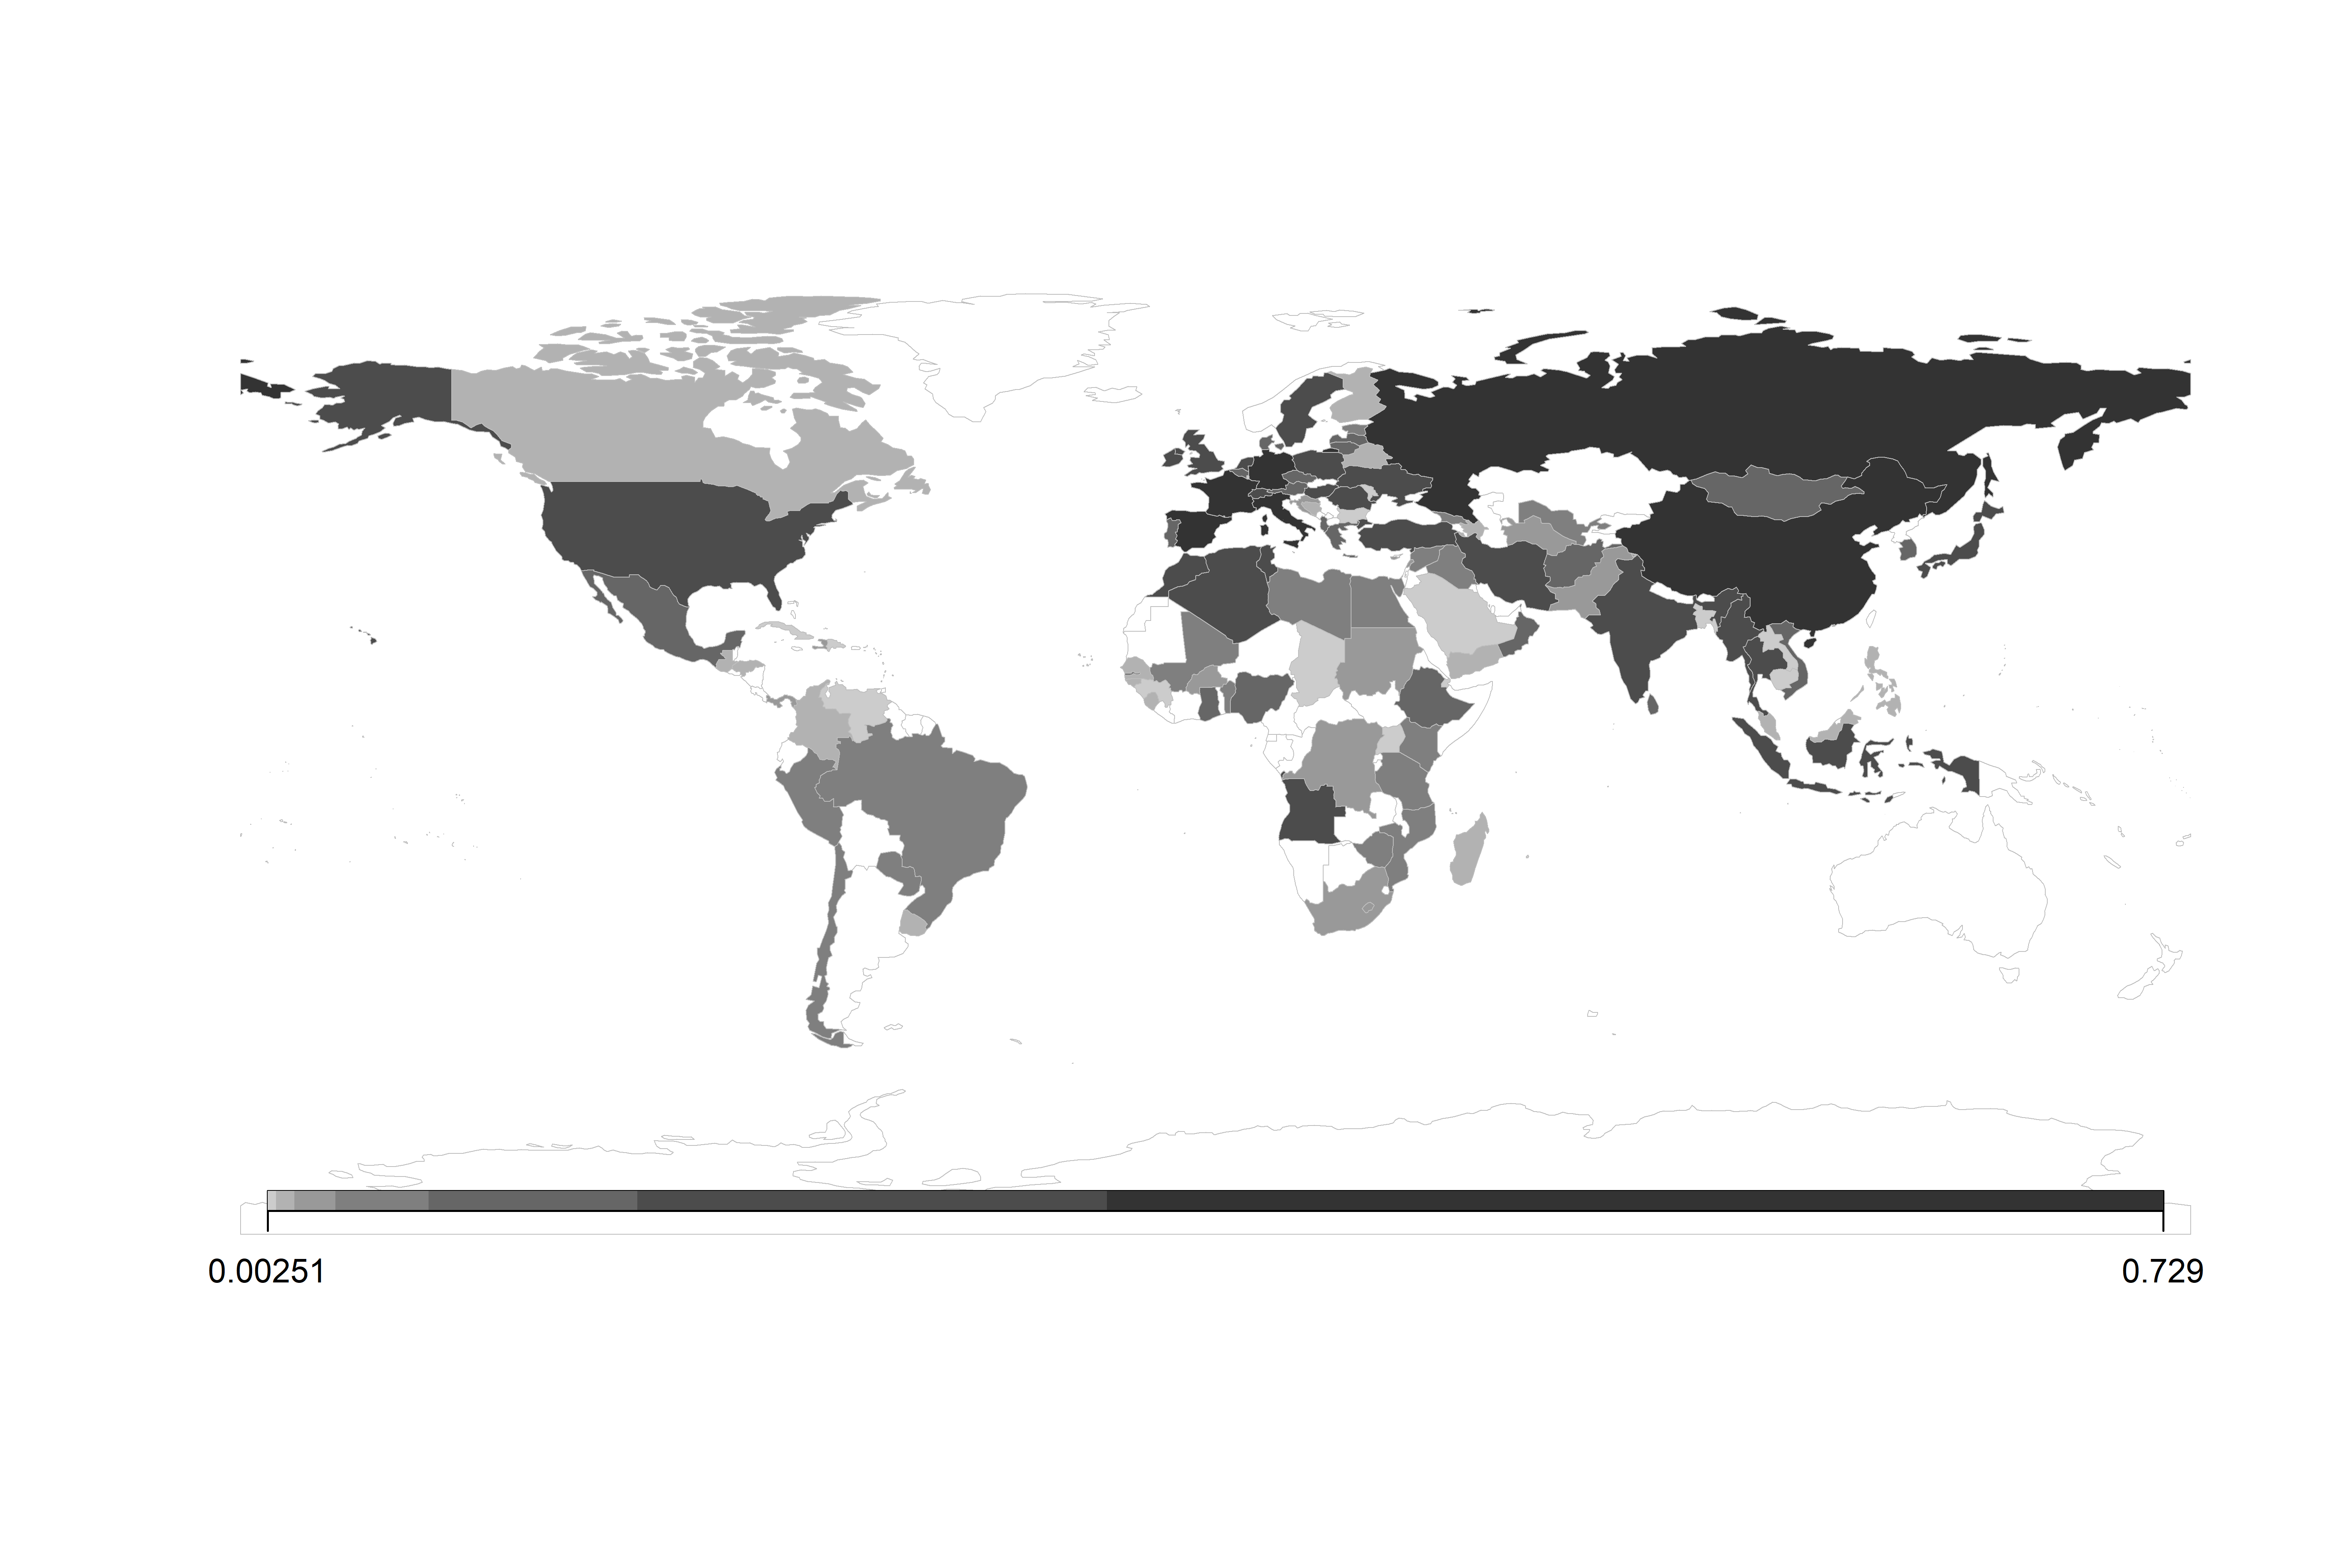
\includegraphics[width=\textwidth,
    height=\textheight, keepaspectratio]{img/historical_conflict_map.png} \caption{Historical Conflict (logged), 1400-1799} \label{Fig: BreckeMap} \end{figure}

In the main models we use the percentage of years between 1400 and 1700 as the main control, but here we test additional specifications. First, we use the raw number of conflicts in a country between 1400-1700. Second, we test the square root transformation of this variable to reduce the impact of outliers. Third, we test the square root transformed percentage of years between 1400-1700 and fourth we test the percentage of conflict years between 1400-\textbf{1799} to assess whether adding 18th century conflicts changes the results. Finally, we interact our main historical conflict control with the region fixed effects, to allow the impacts of war to vary across regions, as \citet{Dincecco2019} find in relation to state capacity. Table \ref{Tab: Hist_Conflict_Rob} shows the results of these models. Our main results are largely unchanged. Similar to \citet{Dincecco2019}, we find that historical conflict in Africa has has a significantly different association with modern conflict than in other regions. 

     
\begin{table}[H]
\begin{center}
\scalebox{0.7}{
\begin{tabular}{l c c c c c}
\hline
 & Model 1 & Model 2 & Model 3 & Model 4 & Model 5 \\
\hline
Log ISD states                                         & $0.03^{**}$ & $0.03^{**}$ & $0.02^{*}$  & $0.03^{**}$ & $0.02^{*}$     \\
                                                       & $(0.01)$    & $(0.01)$    & $(0.01)$    & $(0.01)$    & $(0.01)$       \\
Log mean EPR groups                                    & $0.04^{**}$ & $0.04^{**}$ & $0.03^{**}$ & $0.03^{**}$ & $0.03^{**}$    \\
                                                       & $(0.01)$    & $(0.01)$    & $(0.01)$    & $(0.01)$    & $(0.01)$       \\
Log population density in 1500                         & $0.00$      & $0.01$      & $-0.00$     & $0.00$      & $0.00$         \\
                                                       & $(0.01)$    & $(0.01)$    & $(0.01)$    & $(0.01)$    & $(0.01)$       \\
Former colony                                          & $-0.00$     & $-0.01$     & $0.01$      & $0.00$      & $0.00$         \\
                                                       & $(0.02)$    & $(0.02)$    & $(0.02)$    & $(0.02)$    & $(0.02)$       \\
Historical conflict                                    & $-0.03$     &             &             &             & $-0.05$        \\
                                                       & $(0.07)$    &             &             &             & $(0.12)$       \\
Neolithic revolution                                   & $0.00$      & $0.00$      & $0.00$      & $0.00$      & $0.00$         \\
                                                       & $(0.00)$    & $(0.00)$    & $(0.00)$    & $(0.00)$    & $(0.00)$       \\
Area                                                   & $0.00$      & $0.00$      & $-0.00$     & $0.00$      & $0.00$         \\
                                                       & $(0.00)$    & $(0.00)$    & $(0.00)$    & $(0.00)$    & $(0.00)$       \\
Ethnic fractionalization                               & $0.00$      & $-0.01$     & $0.01$      & $0.00$      & $0.01$         \\
                                                       & $(0.03)$    & $(0.03)$    & $(0.03)$    & $(0.03)$    & $(0.03)$       \\
Log exported slaves by land area                       & $0.00$      & $0.00$      & $0.00$      & $0.00$      & $-0.00$        \\
                                                       & $(0.00)$    & $(0.00)$    & $(0.00)$    & $(0.00)$    & $(0.00)$       \\
Latin America and the Caribbean                        & $0.02$      & $0.02$      & $0.02$      & $0.02$      & $0.03$         \\
                                                       & $(0.03)$    & $(0.03)$    & $(0.03)$    & $(0.03)$    & $(0.03)$       \\
The Middle East and North Africa                       & $0.03$      & $0.04$      & $0.03$      & $0.03$      & $0.01$         \\
                                                       & $(0.02)$    & $(0.02)$    & $(0.02)$    & $(0.02)$    & $(0.03)$       \\
Sub-Saharan Africa                                     & $0.02$      & $0.03$      & $0.03$      & $0.02$      & $0.02$         \\
                                                       & $(0.03)$    & $(0.03)$    & $(0.03)$    & $(0.03)$    & $(0.03)$       \\
Western Europe and North America                       & $-0.01$     & $-0.02$     & $-0.01$     & $-0.01$     & $0.00$         \\
                                                       & $(0.02)$    & $(0.02)$    & $(0.02)$    & $(0.02)$    & $(0.03)$       \\
Asia and Pacific                                       & $0.05^{*}$  & $0.06^{*}$  & $0.05^{*}$  & $0.05^{*}$  & $0.05^{\cdot}$ \\
                                                       & $(0.02)$    & $(0.02)$    & $(0.02)$    & $(0.02)$    & $(0.03)$       \\
Log absolute latitude                                  & $0.00$      & $0.00$      & $0.00$      & $0.00$      & $0.00$         \\
                                                       & $(0.01)$    & $(0.01)$    & $(0.01)$    & $(0.01)$    & $(0.01)$       \\
Log historical conflict                                &             &             &             & $-0.00$     &                \\
                                                       &             &             &             & $(0.09)$    &                \\
No. historical conflicts                               &             & $-0.00$     &             &             &                \\
                                                       &             & $(0.00)$    &             &             &                \\
Log no. historical conflicts                           &             &             & $0.01$      &             &                \\
                                                       &             &             & $(0.01)$    &             &                \\
Historical conflict X Latin America and the Caribbean  &             &             &             &             & $-0.24$        \\
                                                       &             &             &             &             & $(0.43)$       \\
Historical conflict X MENA                             &             &             &             &             & $0.27$         \\
                                                       &             &             &             &             & $(0.20)$       \\
Historical conflict X  Sub-Saharan Africa              &             &             &             &             & $0.82^{**}$    \\
                                                       &             &             &             &             & $(0.29)$       \\
Historical conflict X Western Europe and North America &             &             &             &             & $-0.04$        \\
                                                       &             &             &             &             & $(0.14)$       \\
Historical conflict X Asia and Pacific                 &             &             &             &             & $0.05$         \\
                                                       &             &             &             &             & $(0.12)$       \\
\hline
R$^2$                                                  & $0.32$      & $0.33$      & $0.33$      & $0.32$      & $0.37$         \\
Adj. R$^2$                                             & $0.24$      & $0.25$      & $0.25$      & $0.24$      & $0.27$         \\
Num. obs.                                              & $151$       & $151$       & $151$       & $151$       & $151$          \\
\hline
\multicolumn{6}{l}{\scriptsize{Reference region is Eastern Europe and Central Asia.}}
\end{tabular}
}
\caption{Historical conflict controls}
\label{Tab: Hist_Conflict_Rob}
\end{center}
\end{table}


\clearpage

\subsubsection{Using Project Mars}

Systematically collected data on historical conflict with global coverage are rare, and Brecke's conflict catalogue and \citet{Dincecco2019}'s adaptation are the only source that we are aware of with coverage before 1800. Coverage in the 19th century is better where there are several sources that record wars during this period. Here we draw upon Project Mars (v1.1, \citep{Lyall2020}) to construct an alternative measure of historical conflict. The Project Mars data provide information on 826 different participants in conventional wars from 1800-2011. First, we subsetted the data, including only participants in wars from 1800-1900 and only participants within 1000km of the staring battle. Put differently, we are only including wars in the 19th century and only ``local'' participants in those wars.\footnote{The results are very similar if we use smaller distance thresholds, specifically, 500km and 100km} This excludes cases that would attribute a historical conflict to the United Kingdom when it was fighting in sub-Saharan Africa, for example. We then matched these participating states in Project Mars with states in the ISD data using the Statename variable. Then, we have coded the modern ``destination states'' for each participant using the information in ISD on the modern locations of ISD states. For states in \citet{Lyall2020} without a matching ISD state, we have coded the modern state in which the participant was located. For each modern state, we then calculated the total number of historical wars that involved a state on that territory. For example, if all participants in a historical war (as indicated by \textit{warnum} in \citet{Lyall2020}) were within the territory of a single modern state, that territory is attributed with one historical war. For example, the Tukolor-Bambara war of 1855 (\textit{warnum} 75) involves the Tukolor empire and the kingdom of Kaarta, both primarily based in modern day-Mali. This conflict started 425km from the capital of Tukolor and 1km from Kaarta and therefore both are retained as ``local'' participants. Since both participants are located in modern Mali, Mali is attributed with the historical conflict. Some conflicts involve ``local'' participants located in different modern states. For example the Durrani Empire and the Sikh Kingdom fought several wars between 1813 and 1822. The Durrani Empire is in modern day Afghanistan and the Sikh empire in modern-day Pakistan. Both of these states were ``local'' participants, located less than 1000km from the starting battle, and in this case, both Afghanistan and Pakistan are attributed with a historical conflict.       

This approach to measuring historical conflict has some advantages. Primarily, wars in Project Mars are linked to specific states in the ISD, meaning that if our results are best explained by historical states fighting wars then there is a closer conceptual link between states and wars using these data. Brecke, for example, includes wars that may not involve states and are less relevant to explaining the HSE-conflict link we outline in the paper. 

The main downside is that this measure introduces post-treatment bias because the wars are measured contemporaneously to statehood (i.e between 1800-1900). More wars probably occur in territories with more states to fight them and to the extent that states cause wars we are controlling for part of the association between HSEs and modern conflict. Empirically this appears to be the case as both the historical conflict indicator from \citet{Dincecco2019} and the measure based on \citet{Lyall2020} are highly correlated with the number of HSEs. Table \ref{Tab: Hist_Conf_Models} shows some simple associations between the levels of historical conflict and the number of HSEs, controlling for population density in 1500, the timing of the neolithic revolution, land area, latitude and slave exports by land area. 

     
\begin{table}[H]
\begin{center}
\scalebox{0.7}{
\begin{tabular}{l c c}
\hline
 & Brecke Conflicts 1400-1799 & Project Mars 19th C. Wars \\
\hline
Log ISD states                   & $0.02^{*}$   & $0.28^{***}$ \\
                                 & $(0.01)$     & $(0.08)$     \\
Log population density in 1500   & $0.04^{***}$ & $0.04$       \\
                                 & $(0.01)$     & $(0.04)$     \\
Neolithic revolution             & $-0.00$      & $0.00$       \\
                                 & $(0.00)$     & $(0.00)$     \\
Area                             & $0.03^{***}$ & $0.07^{*}$   \\
                                 & $(0.00)$     & $(0.03)$     \\
Log exported slaves by land area & $-0.00$      & $0.01$       \\
                                 & $(0.00)$     & $(0.02)$     \\
Log absolute latitude            & $0.02^{**}$  & $0.04$       \\
                                 & $(0.01)$     & $(0.06)$     \\
\hline
R$^2$                            & $0.49$       & $0.16$       \\
Adj. R$^2$                       & $0.47$       & $0.12$       \\
Num. obs.                        & $152$        & $152$        \\
\hline
\multicolumn{3}{l}{\scriptsize{$^{***}p<0.001$; $^{**}p<0.01$; $^{*}p<0.05$; $^{\cdot}p<0.1$}}
\end{tabular}
}
\caption{Historical conflict and historical states}
\label{Tab: Hist_Conf_Models}
\end{center}
\end{table}


Symbols and institutions, for example, could be more potent or established when historical states have a history of fighting conventional wars. Nonetheless, the historical conflict- modern conflict link is an alternative mechanism to our proposed mechanism and this approach represents an alternative method to account for the impacts of historical conflict that complements the analyses with the Brecke data. 

Figure \ref{Fig: Mars_Map} shows the spatial distribution of wars in the 19th century, using the data from \citet{Lyall2020}. 

   \begin{figure}[H] \hspace{-0,5cm} 
   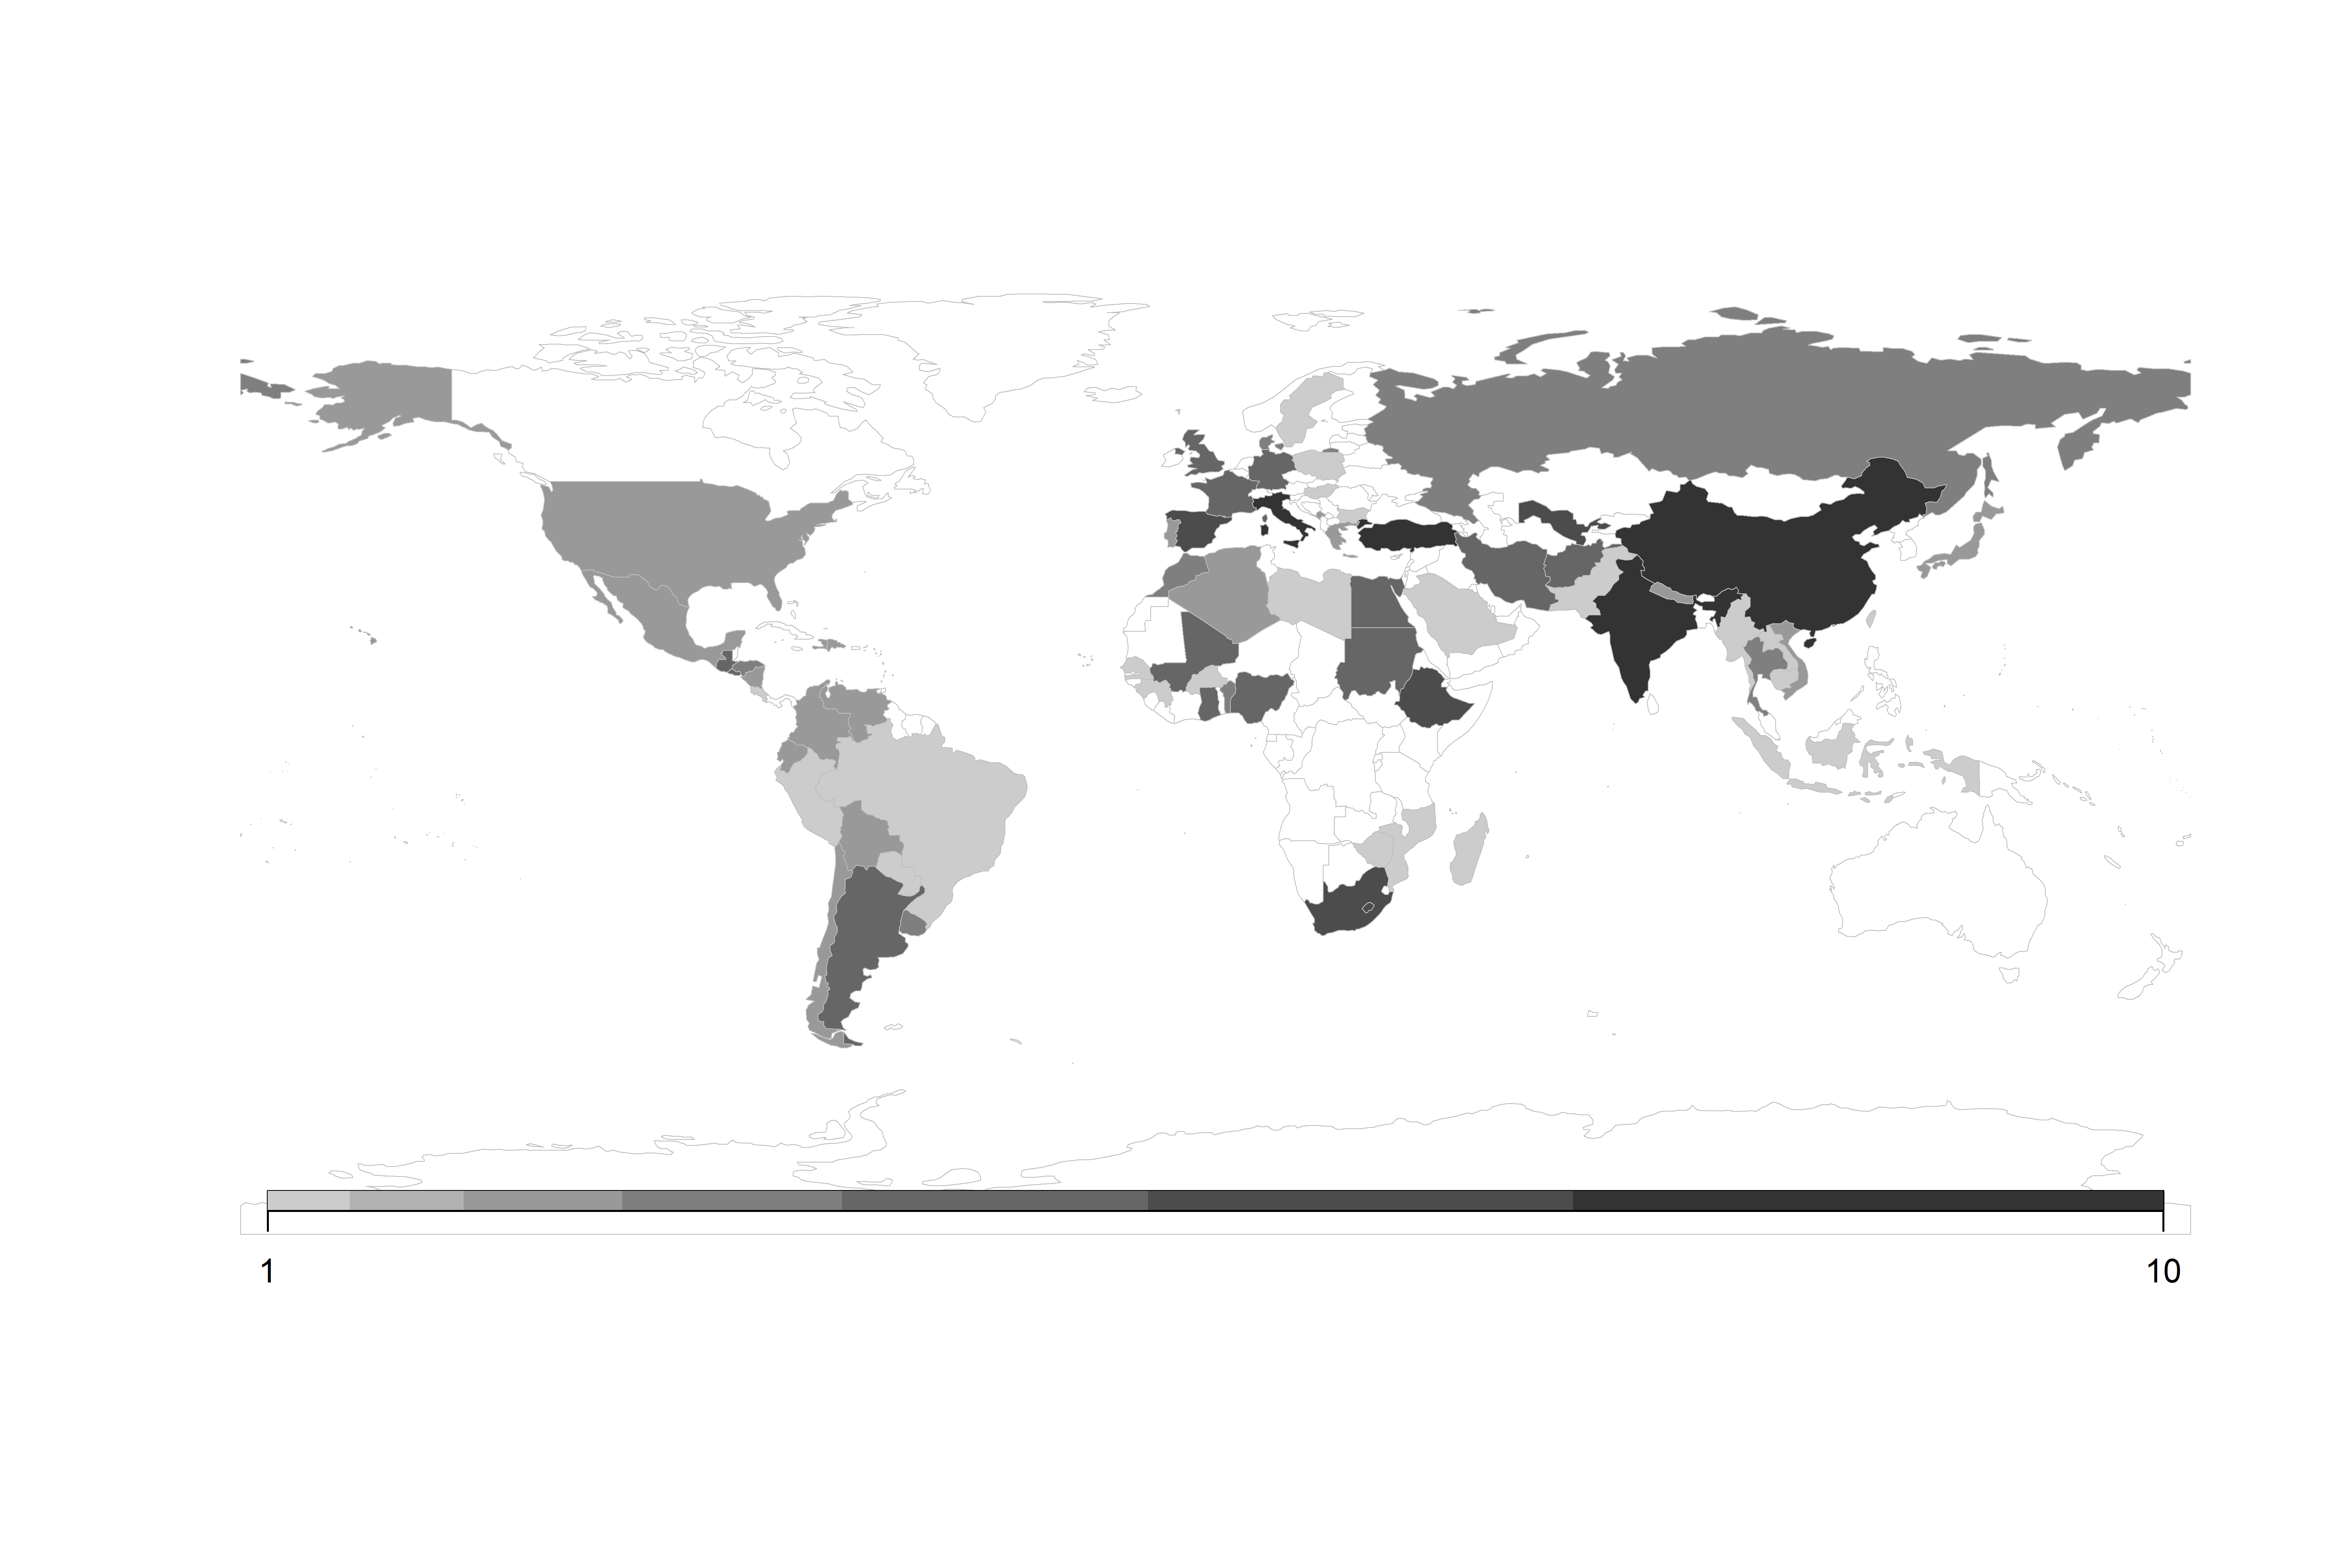
\includegraphics[width=\textwidth,
    height=\textheight, keepaspectratio]{img/historical_conflict_pm_map.png} \caption{Historical Conflict in Project Mars (logged), 1800-1900} \label{Fig: Mars_Map} \end{figure}


Table \ref{Tab: Hist_Conflict_Rob_Pm} shows the main results replacing the historical conflict indicator used in the main analysis with the indicator of 19th century wars from \citet{Lyall2020}. 

     
\begin{table}[H]
\begin{center}
\scalebox{0.7}{
\begin{tabular}{l c c c c}
\hline
 & Model 1 & Model 2 & Model 3 & Model 4 \\
\hline
Log ISD states                        & $0.03^{**}$ & $0.03^{**}$ & $0.03^{**}$ & $0.03^{**}$ \\
                                      & $(0.01)$    & $(0.01)$    & $(0.01)$    & $(0.01)$    \\
Log mean EPR groups                   & $0.03^{**}$ & $0.03^{**}$ & $0.03^{**}$ & $0.03^{**}$ \\
                                      & $(0.01)$    & $(0.01)$    & $(0.01)$    & $(0.01)$    \\
Log population density in 1500        & $0.00$      & $0.00$      & $0.00$      & $0.00$      \\
                                      & $(0.01)$    & $(0.01)$    & $(0.01)$    & $(0.01)$    \\
Former colony                         & $0.00$      & $0.00$      & $0.00$      & $0.00$      \\
                                      & $(0.02)$    & $(0.02)$    & $(0.02)$    & $(0.02)$    \\
Neolithic revolution                  & $0.00$      & $0.00$      & $0.00$      & $0.00$      \\
                                      & $(0.00)$    & $(0.00)$    & $(0.00)$    & $(0.00)$    \\
Area                                  & $0.00$      & $0.00$      & $0.00$      & $0.00$      \\
                                      & $(0.00)$    & $(0.00)$    & $(0.00)$    & $(0.00)$    \\
Ethnic fractionalization              & $0.00$      & $0.00$      & $0.00$      & $0.00$      \\
                                      & $(0.03)$    & $(0.03)$    & $(0.03)$    & $(0.03)$    \\
Log exported slaves by land area      & $0.00$      & $0.00$      & $0.00$      & $0.00$      \\
                                      & $(0.00)$    & $(0.00)$    & $(0.00)$    & $(0.00)$    \\
Latin America and the Caribbean       & $0.02$      & $0.01$      & $0.02$      & $0.01$      \\
                                      & $(0.03)$    & $(0.03)$    & $(0.03)$    & $(0.03)$    \\
The Middle East and North Africa      & $0.03$      & $0.03$      & $0.03$      & $0.03$      \\
                                      & $(0.03)$    & $(0.02)$    & $(0.02)$    & $(0.02)$    \\
Sub-Saharan Africa                    & $0.02$      & $0.02$      & $0.02$      & $0.02$      \\
                                      & $(0.03)$    & $(0.03)$    & $(0.03)$    & $(0.03)$    \\
Western Europe and North America      & $-0.01$     & $-0.01$     & $-0.01$     & $-0.01$     \\
                                      & $(0.02)$    & $(0.02)$    & $(0.02)$    & $(0.02)$    \\
Asia and Pacific                      & $0.05^{*}$  & $0.05^{*}$  & $0.05^{*}$  & $0.05^{*}$  \\
                                      & $(0.03)$    & $(0.02)$    & $(0.03)$    & $(0.03)$    \\
Log absolute latitude                 & $0.00$      & $0.00$      & $0.00$      & $0.00$      \\
                                      & $(0.01)$    & $(0.01)$    & $(0.01)$    & $(0.01)$    \\
Log no. 19th C Wars                   & $-0.00$     &             &             &             \\
                                      & $(0.01)$    &             &             &             \\
Log no. 19th C Wars (500km threshold) &             & $0.00$      &             &             \\
                                      &             & $(0.01)$    &             &             \\
Log 19th C war-participant war-days   &             &             & $-0.00$     &             \\
                                      &             &             & $(0.00)$    &             \\
Log 19th C war KIA                    &             &             &             & $0.00$      \\
                                      &             &             &             & $(0.00)$    \\
\hline
R$^2$                                 & $0.32$      & $0.32$      & $0.32$      & $0.32$      \\
Adj. R$^2$                            & $0.24$      & $0.24$      & $0.24$      & $0.24$      \\
Num. obs.                             & $151$       & $151$       & $151$       & $151$       \\
\hline
\multicolumn{5}{l}{\scriptsize{Reference region is Eastern Europe and Central Asia.}}
\end{tabular}
}
\caption{Historical conflict controls (using Project Mars)}
\label{Tab: Hist_Conflict_Rob_Pm}
\end{center}
\end{table}


\clearpage

\subsubsection{Conclusions}

The preceding discussion leads us to conclude that historical conflict does not confound our main results, at least as far as we can empirically test that with the measures available. More historical states \textit{are} correlated with more historical conflicts, but historical conflicts do not appear to be strongly correlated with modern armed conflicts. This is likely because wars in the past have conditional effects on state-building and future peace. Some wars, especially those in Europe, probably helped create cohesive, modern states that had overcome important state-building challenges prior to the 20th century. Here, past wars may be associated with future peace. But in other regions, primarily Africa, historical wars may have eroded trust between social groups that transmits into the modern world as weaker states and higher conflict risks \citep{Besley2014, Dincecco2019}. Our results reflect this - only in Africa do we find that historical conflict is correlated with modern conflict. Historical states may be correlated with historical wars, but they don't appear to be strongly correlated with modern wars. Nonetheless, when we do allow the impacts of war to vary by region, our main results hold up, suggesting that even in Africa, historical warfare and historical statehood may have different impacts on the propensity to modern conflict. 




\subsection{Table of cases}
 
 % latex table generated in R 4.1.2 by xtable 1.8-4 package
% Wed Jan 26 12:09:38 2022
\begin{xltabular}{\textwidth}{p{0.1\textwidth}p{0.15\textwidth}p{0.1\textwidth}p{0.1\textwidth}p{0.5\textwidth}}
  \toprule
Country & Actor & Onset year(s) & Mechanism & Narrative \\ 
  \midrule
Ethiopia & ALF & 1975-1991 & Networks & State tried to curtail traditional Sultanate \citep{Shehim1985}. \\ 
  Uganda & Buganda & 1966 & Networks & Power sharing agreement broke down leading to a breif civil war \citep{Tuck2005}. \\ 
  DR Congo & State of Katanga & 1961 & Networks & Formal institution (king) led bid for secession of the Katanga region. \citep[99-100]{Nzongola2002} \\ 
  DR Congo & BDK & 1989 & Symbols &  \\ 
  DR Congo & Mining State of South Kasai & 1960 & Networks, symbols & Traditional chief led secession movement of South-Kasai region, and resurrected the royal title of the Luba Empire. \citep[105]{Nzongola2002} \\ 
  Indonesia & GAM & 1976 & Networks & Networks with deep roots to the HSE of Aceh used for rebel recruitment \citep{Aspinall2009}. \\ 
  Mali & FLM & 2015 & Symbols & The name of the group refers to an HSE \citep{Brown1968}. \\ 
  Mali & MUJWA & 2011 & Symbols & The groups seeks to revive the jihad of a HSE \citep{Zenn2015}. \\ 
  Nigeria & Ansaru & 2009 & Symbols & The groups seeks to revive the jihad of a HSE \citep{Zenn2015}. \\ 
  Libya & CLA & 2012 & Networks, symbols & The groups name refers to a short lived kingdom in Eastern Libya and the group elected a descendent of the former king as their leader \citep{Ahram2019}. \\ 
  India & ULFA & 1979 & Symbols & The group frequently invokes the Ahom kingdom and the chairman claims to be a prince eligible for the long defunct royal title \citep{Mahanta_2013, Goswami2014} \\ 
  India & UNLF, KCP, PREPAK  & 1979 & Symbols & Manipuri insurgent groups used the name of the historical kingdom (Kangleipak) and fought against the ``forced merger'' of between India and the princely state of Manipur \citep{Pettersson2021} \\ 
  Pakistan & BLF, BLA & 1948, 1974, 2004, 2019 & Symbols, networks & Low scale insurgency following forced accession of the Khan of Kalat. Khan redeclared independence in 1958, and the new khan announced the creation of the Council of Independent Balochistan in 2009 \citep{Ahmad2017} \\ 
    China & ETIM & 2008 & Symbols &  East Turkistan Islamic Movement (ETIM) seeks to revive the historical state of East Turkistan \citep{Pettersson2021, Soloshcheva2017} \\ 	  
    China & Tibet & 1950, 1956, 1959 & Symbols, networks &  Tibetan insurgents aim to restore the independence of the historical state of Tibet \citep{Pettersson2021} \\ 
    India & Sikh insurgents & 1983 & Symbols &  Sikhs seek to establish the independent state of Khalistan, referring to a long history of Sikh statehood, famously led by Rajit Singh in the 19th century \citep{Pettersson2021} \\ 
    Somalia & SSDF, Puntland & 1982 & Networks & Following the first civil war in Somalia, Puntland declares itself an autonomous region within federal Somalia. The elite has close ties to the old Majeerteen sultanate elite \citep[111-112]{Wimmer2018} \\ 
    Nigeria, CHA & Boko Haram & 2009 & Symbols & Founder of Boko Haram aims to restore Islamic rule with reference to the pre-colonial states of Kanem-Borno and the Sokoto Caliphate \citep{Barkindo2016, Zenn2013}  \\ 
    Malaysia & Sultanate of Sulu & 2013 & Symbols, institutions, networks & Sultanate of Sulu claims historical territory in Sabah, leading to fighting with Malaysia \citep{Pettersson2021}  \\     
    Philippines & MILF & 2013 & Symbols & The Moro Islamic Liberation Front uses the examples of the Sultanate of Maguindanao and the Sultanate of Sulu to justify demands for independence \citep[81]{Tuminez2007}  \\  
    Sudan & Darfuri rebel groups & 2003 & State weakness & Darfuri rebel groups launch an insurgency against the central government in Khartoum. The Darfur region is comparatively weak and undeveloped in part because the historical Sultanate of Darfur was ruled indirectly during colonialism while Khartoum and it's surrounds were the site of colonial state and infrastructure investments \citep[299]{OFahey2008}  \\
   \bottomrule
\end{xltabular}

 
 \pagebreak \bibliographystyle{agsm_mod} \bibliography{ArtificialBorders.bib}
 
\end{document}